\chapter{Resultados}
\label{chap:resultados}

\drop{E}{ste} capítulo se encuentra destinado a exponer los resultados que se han obtenido a partir de la aplicación de la metodología escogida como base en el capítulo anterior.

\section{Análisis estratégico}
La realización de un análisis estratégico resulta de utilidad tanto para las empresas de nueva creación como para las que se encuentran ya asentadas en el mercado, puesto que permite comprender en mayor medida las condiciones en las que opera la empresa en un determinado momento. De esta manera, es posible planificar o prever los movimientos estratégicos para adaptarse a los cambios que pueden haberse producido o que pueden llegar a producirse tanto en el entorno general como en el específico y llevar a cabo cambios en el modelo de negocio. Por tanto, puesto que el marco de este \acs{TFM} es el de la creación de una empresa que provea servicios \acs{DaaS}, esta sección se dedicará a realizar un análisis estratégico para diseñar el modelo de negocio de esta, de manera que se pueda ofrecer un servicio que aporte valor a los clientes de manera adecuada y rentable.

\subsection{Análisis del entorno general}
Uno de los primeros pasos que se deben llevar a cabo es la realización de un análisis PESTEL, que es un modelo que permite la la realización del análisis del entorno general para descubrir las posibles amenazas externas o factores a considerar en la toma de decisiones posterior en cuanto al modelo de negocio. De esta manera, se podrán tener en cuenta las fuerzas políticas, económicas, socio-culturales, tecnológicas, medioambientales o ecológicas y legales. Aunque algunas actúan de manera relativamente aislada o independiente como la medioambiental, la mayoría de estas fuerzas se encuentran interrelacionadas como la socio-cultural, que podría variar en función del estado económico en un determinado instante.

\clearpage

Por tanto, aunque en este caso se realizaría en el momento de la creación de una empresa, se trata de una técnica a realizar de manera periódica con el fin de identificar y anticiparse a los potenciales cambios en el entorno general \cite{jedidiagarciallergo2012}. A continuación, se analizarán los diferentes factores que contempla este análisis, centrándose principalmente en el ámbito territorial de España, así como en los factores políticos de la \acf{UE}, puesto que el Estado Español forma parte de esta como estado miembro desde el año 1985 y como tal, España se ve afectada en cierto modo de las políticas o decisiones que se tomen en ella. 
%Estos dos territorios son los que se espera que se encuentre la operación de la empresa, por lo que se hará una distinción entre ellos en cada uno de los mencionados factores.

\subsubsection{Factores políticos}
Aunque pueda parecer que las decisiones políticas se encuentren en un plano más lejano al de las empresas, la realidad es que, normalmente, las primeras pueden llegar a tener una gran trascendencia en las segundas. Además, las políticas también suelen tener una repercusión legislativa, factor del que se hablará en un capítulo posterior.

\noindent\underline{España}\newline
\indent La forma de gobierno de España \cite{santandertrade} se basa en una monarquía constitucional parlamentaria con un poder descentralizado, debido a la existencia de la división de poderes en poder ejecutivo, legislativo y judicial. Por tanto, puesto que el primer apartado se centra en el análisis de los factores políticos, este punto centrado en el poder ejecutivo.

Al tratarse de una monarquía, el Rey es el Jefe del Estado y el comandante en jefe del Ejército. Por otra parte, al ser una democracia, la elección del Presidente del Gobierno se realiza por medio de unas elecciones legislativas a nivel nacional, donde gobierna el candidato que el Rey ha designado para formar gobierno del partido que ha obtenido la mayoría de votos provenientes de la ciudadanía o, en su defecto, el candidato que ha conseguido aunar una mayor cantidad de apoyos de otros partidos que cuentan con representación en el Congreso de los Diputados, cuya función principal es la de legislar. La duración de una legislatura se encuentra fijada en un máximo de cuatro años en la Constitución, por lo que pasado ese tiempo se deberán celebrar unas nuevas elecciones. De igual manera, se cuenta con un Senado, que se trata de la cámara alta del poder legislativo cuyos representantes son elegidos por la ciudadanía y se encarga de realizar una <<segunda lectura>> de los asuntos tratados en el Congreso.

\clearpage

Además del Gobierno Central, parte de este poder también recae en cada una de las 17 comunidades autónomas, así como en las dos ciudades autónomas en las que se divide el Estado español, donde se cuenta con un presidente. Al igual que sucede en el Gobierno Central, este presidente es el candidato con la mayor cantidad de votos de los ciudadanos o el que ha conseguido un mayor número de apoyos dentro del parlamento autonómico y las elecciones son celebradas cada cuatro años, como máximo.

Actualmente, en el momento de la realización de este análisis y desde hace algunos años, se cuenta con una situación política diferente, cuyo principal defecto es un considerable grado de inestabilidad. Esto hace que organismos como el Banco de España duden de la economía Española y avisen de que la política económica y fiscal del Gobierno, al no estar formado aún, pueda debilitarse y entrar en una cierta desaceleración, como se refleja en la Figura \ref{fig:evolrazon} \cite{larazon2019}.

\begin{figure}[h]
  \centering
  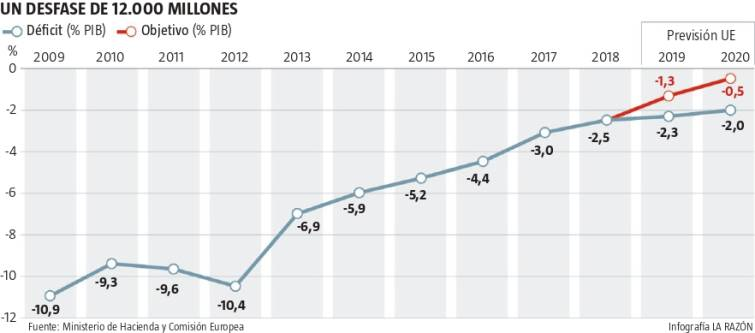
\includegraphics[width=0.9\linewidth]{figures/images/evolucion_larazon.jpg}
  \caption{Previsiones de evolución económica}
  \label{fig:evolrazon}
\end{figure}

En cuanto a la capacidad emprendedora de España, según el informe \acf{GEM} España, publicado en este año 2019 \cite{informegem2019}, la \acf{TEA} ha subido hasta un 6,4\% en el pasado año donde las políticas gubernamentales ostentan el sexto puesto en cuanto a obstáculos se refiere. Según los expertos, esto es debido al exceso de burocracia, impuestos elevados y diferente regulación según la comunidad autónoma \cite{yolandagonzalez2019}, lo que también representaría una cierta amenaza. No obstante, estos expertos valoraron de manera positiva a nuestro país con respecto a las iniciativas gubernamentales de impulso al emprendimiento y las infraestructuras con las que se cuenta.

\clearpage

Por otra parte, en lo que concierne a la política laboral, actualmente existen algunos choques entre varias partes \cite{manuelvgomez2019}. La última reforma laboral fue aprobada hace siete años aunque los sindicatos y algunos partidos políticos piden cambiarla, mientras que otros partidos y la \acf{CEOE} lo rechazan. Esta reforma, principalmente, iba enfocada a reducir la precariedad laboral creciente que tenía el país en el año 2012, aunque no fue capaz de ponerle fin definitivamente. A pesar de esto, aunque no se ha solucionado ese problema, actualmente se cuenta con un mayor número de puestos de trabajo.

Finalmente, algunos aspectos del ámbito político se presentan favorables a un impulso en el desarrollo de la educación en su ámbito digital. Recientemente, Pedro Sánchez Pérez-Castejón, entonces Presidente del Gobierno en funciones, comunicó los cuatro ejes principales de la propuesta de Gobierno \cite{tweetsanchez2019}, entre los que se encuentra lo que ha denominado como <<digitalización de la economía y la educación>> (Figura \ref{fig:tweetsanchez}).

\begin{figure}[h]
  \centering
  
\includegraphics[width=0.8\linewidth]{figures/images/tweet_sanchez.png}
  \caption{\textit{Tweet} de Pedro Sánchez}
  \label{fig:tweetsanchez}
\end{figure}

\clearpage

\noindent\underline{\acs{UE}}\newline
\indent Por lo que a la \acs{UE} respecta, se cuenta con la presencia de un Parlamento Europeo \cite{parlamentoue}, el Consejo de la Unión Europea \cite{consejoue}, el Consejo Europeo \cite{consejoeuropeo} y la Comisión Europea \cite{comisionue}. 

La principal función del Parlamento Europeo es la de ostentar las responsabilidades legislativas, de supervisión y presupuestarias. Se elige mediante votación de los ciudadanos de la \acs{UE} cada cinco años y, al igual que ha sucedido en España, se han celebrado elecciones recientemente, en mayo del 2019. Entre sus competencias legislativas se encuentra la de aprobar la legislación de la \acs{UE} junto con el Consejo de la \acs{UE} a partir de las propuestas de la Comisión Europea.

El Consejo de la \acs{UE} tiene como principal función representar a los Gobiernos de los Estados miembros, adoptar la legislación europea y coordinar las políticas de la \acs{UE}. Se encuentra formado por los ministros de cada país de la \acs{UE}, dependiendo del tema que se vaya a tratar. Junto con el Parlamento Europeo es el principal órgano de decisión.

El Consejo Europeo es una institución que reúne a los líderes de la \acs{UE} en cumbres trimestrales donde se definen la orientación y las prioridades de las políticas generales de la \acs{UE}. Está formado por los Jefes de Estado o Gobierno de cada país y los presidentes del Consejo Europeo y de la Comisión Europea. Por tanto, representa el nivel más elevado de cooperación política, aunque carece de la capacidad de legislar.

Por último, la Comisión Europea tiene como función principal la de velar por los intereses generales proponiendo y comprobando el cumplimiento de la legislación vigente y aplicando las políticas y el presupuesto de la \acs{UE}. Está formada por un conjunto de comisarios, donde cada uno de ellos actúa en representación de su país. Se trata del órgano ejecutivo políticamente independiente de la \acs{UE}, responsable de la elaboración de las propuestas de nuevas leyes y de aplicar las decisiones del Parlamento Europeo y del Consejo de la \acs{UE}.

Por otra parte, si en el caso de España la \acs{TEA} se situaba en el 6,4\%, según el informe \acs{GEM} Global publicado en este año 2019 \cite{informegemglobal}, el promedio europeo se encuentra en un 8,7\%.

Teniendo todo esto en cuenta, a pesar de que las elecciones se han celebrado recientemente, ya se ha constituido el Parlamento Europeo y se ha elegido un presidente. No obstante, los cambios en las políticas en este caso suelen llevar más tiempo debido a la implicación de un mayor número de partes. Por ejemplo, el \acf{RGPD}, del que se hablará más adelante, fue aprobado en el año 2016 aunque no fue hasta dos años después cuando entró en vigor. Por lo tanto, se considera que en los próximos cinco años podría haber cierta estabilidad dentro de la \acs{UE}.

\clearpage

\subsubsection{Factores económicos}
Los factores económicos engloban todo lo relacionado con las cuestiones económicas y su posible impacto en el desarrollo normal de la empresa.

\noindent\underline{Empleo}\newline
\indent Recientemente, la economía española ha pasado por una crisis que comenzó en el año 2008 terminando, oficialmente, en 2014. Durante esos años, indicadores como la tasa de desempleo, el \acf{PIB} o el \acf{IPC} empeoraron sus valores y, con estos y otros sucesos, la economía se vio resentida. A continuación, se realizará un estudio de los indicadores y valores económicos más importantes.

Comenzando con la tasa de paro, se puede observar su evolución desde enero de 2007 hasta junio de 2019 en la Figura \ref{fig:tasaparo}. Desde mediados de 2007 comienza a subir, pero no es hasta 2008 cuando esa subida comienza a ser más acusada. Desde entonces, continuó su aumento hasta marzo del año 2013, donde alcanzó un máximo absoluto en 5.035.243 parados. A partir de entonces, la cifra comenzó a disminuir progresivamente presentando algunas fluctuaciones propias de las épocas del año hasta situarse en 3.015.686 parados en junio de 2019. Por tanto, este indicador sería uno de los más favorables dentro de este apartado.

\begin{figure}[h]
  \centering
  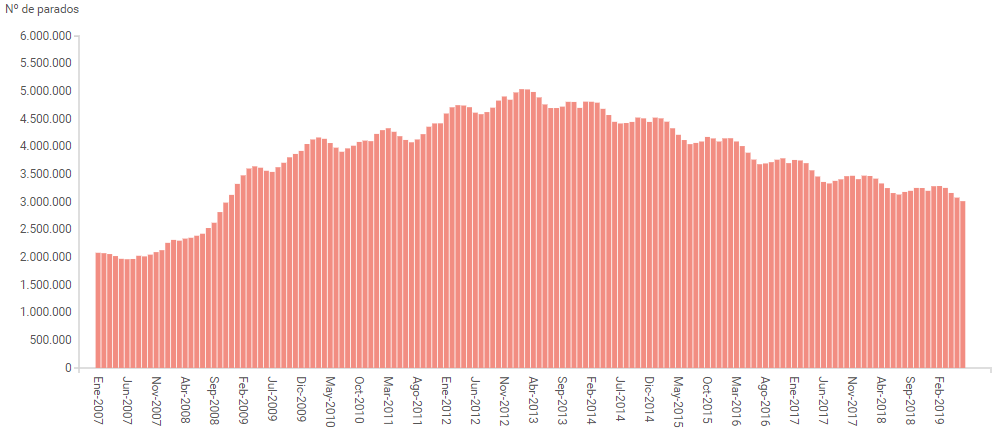
\includegraphics[width=0.9\linewidth]{figures/images/evolucion_paro.PNG}
  \caption{Evolución de la tasa de paro en España (2007-2019)}
  \source{Ministerio de Empleo y Seguridad Social}
  \label{fig:tasaparo}
\end{figure}

\clearpage

\noindent\underline{\acs{PIB}}\newline
\indent En cuanto al \acs{PIB}, este indicador representa la riqueza de un país a lo largo de un periodo determinado. Según sus valores \cite{pibexpansion}, ha crecido un 0,7\% durante el primer trimestre de 2019, en comparación con el anterior trimestre, acumulando porcentajes de crecimiento de entre el 1,4\% y el 2,6\% interanuales desde el año 2014 (Tabla \ref{tab:evo_pib}). Al igual que sucede con la tasa de paro, este indicador podría formar parte de los indicadores favorables para la creación de empresas.

\begin{table}[!htbp]
	\centering
	{\small
		\begin{tabular}{|c|c|c|}
\hline
\rowcolor[HTML]{343434} 
\multicolumn{3}{|c|}{\cellcolor[HTML]{343434}{\color[HTML]{FFFFFF} \textbf{Evolución \acs{PIB} anual España}}}                                                                                                                                                    \\ \hline
\rowcolor[HTML]{9B9B9B} 
\multicolumn{1}{|l|}{\cellcolor[HTML]{9B9B9B}{\color[HTML]{FFFFFF} \textbf{Año}}} & \multicolumn{1}{l|}{\cellcolor[HTML]{9B9B9B}{\color[HTML]{FFFFFF} \textbf{\acs{PIB} anual (M. \euro)}}} & \multicolumn{1}{l|}{\cellcolor[HTML]{9B9B9B}{\color[HTML]{FFFFFF} \textbf{Var. PIB (\%)}}} \\ \hline
2018    & 1.208.248    &    2,6    \\ \hline
2017    & 1.166.319    & 3,0    \\ \hline
2016    & 1.118.743    & 3,2    \\ \hline
2015    & 1.081.165    & 3,6    \\ \hline
2014    & 1.037.820    & 1,4    \\ \hline
2013    & 1.025.693    & -1,7   \\ \hline
2012    & 1.039.815    & -2,9   \\ \hline
\end{tabular}
	}
	\caption[Evolución del \acs{PIB} en España]
	{Evolución del \acs{PIB} en España}
	\label{tab:evo_pib}
\end{table}

\noindent\underline{Impuestos}\newline
\indent A pesar de que los dos indicadores anteriores podrían parecer favorables a la creación de una empresa, tanto estas como las personas físicas han de tributar una serie de impuestos a la Hacienda Pública, por lo que deberán ser tenidos en cuenta en el desarrollo de la actividad empresarial, financiación y rentabilidad. En cuanto a la clasificación de los impuestos en España, existen dos tipos \cite{balcellsg}: directos e indirectos. Mientras que los primeros se tributan en función de la renta o patrimonio de las personas o entidades, los segundos se aplican sobre transacciones, gravando servicios o bienes. Por otra parte, también existe la clasificación por impuestos para autónomos y personas físicas y los impuestos para sociedades.

Comenzando por los impuestos directos, el \acf{IRPF} grava la renta de las personas y se trata de un impuesto progresivo, que aumenta o disminuye en función de la cantidad de dinero percibida y, por tanto, mide la capacidad contributiva de estas, variando entre comunidades autónomas y teniendo en cuenta una gran cantidad de factores.

En cuanto al impuesto sobre las ganancias de capital, se trata de un impuesto que se ha de afrontar al vender una propiedad por encima de su valor de adquisición y se encuentra entre el 19\% y el 23\%. El \acf{IP} varía entre el 0,2\% y el 2,5\% y se paga en función de los activos o riquezas que se posean. En cuanto al \acf{ISD}, se debe pagar cuando se realiza un traspaso de titularidad debido a una herencia o donación, variando entre comunidades autónomas. Uno de los principales impuestos con los que se lidia prácticamente a diario es el \acf{IVA} \cite{impuestosautonomo}, que recae en el consumidor, mientras que la empresa deberá tributar la diferencia entre el \acs{IVA} cobrado a los clientes y el que hayan tenido que pagar a sus proveedores. Este impuesto se paga cada tres meses y en España existen tres tipos: estándar (21\%), reducido (10\%) y súper-reducido (4\%). Por último, el \acf{IRNR} grava la renta de las personas que no residen dentro del territorio español, viviendo menos de 183 días por año. 

Por otra parte, en cuanto a los impuestos para sociedades, se encuentra el \acf{IS}, que es un impuesto directo que grava en un 25\% los beneficios procedentes de la actividad económica de una empresa. Además, existe también el \acf{ITP}, que grava las operaciones que pueden darse a lo largo de la vida de una empresa, como ampliaciones de capital, fusiones, etc.

Todos estos impuestos deberán ser tenidos en cuenta a la hora de llevar a cabo la creación de una empresa y un correcto desarrollo de la actividad empresarial.

\noindent\underline{Inflación}\newline
\indent La inflación, junto con otros indicadores como el \acf{IPC}, representa la salud de la economía de un territorio. Mientras que el \acs{IPC} es calculado teniendo en cuenta un determinado conjunto de productos, la inflación considera los precios de la economía de manera general. Por tanto, una inflación moderadamente alta indicará el crecimiento positivo de un país y, con ello, el consumo de sus habitantes. Por otra parte, una inflación negativa o baja indicaría un empeoramiento de la economía. En la Tabla \ref{tab:evo_inflacion} se muestran los datos de la inflación en España desde el año 2012, donde se observa que la economía ha ido consolidando un crecimiento constante en los últimos años.

\begin{table}[!htbp]
	\centering
	{\small
		\begin{tabular}{|c|c|}
\hline
\rowcolor[HTML]{343434} 
\multicolumn{2}{|c|}{\cellcolor[HTML]{343434}{\color[HTML]{FFFFFF} \textbf{Evolución inflación anual España}}}                                                                                                                                                    \\ \hline
\rowcolor[HTML]{9B9B9B} 
\multicolumn{1}{|c|}{\cellcolor[HTML]{9B9B9B}{\color[HTML]{FFFFFF} \textbf{Año}}} & \multicolumn{1}{|c|}{\cellcolor[HTML]{9B9B9B}{\color[HTML]{FFFFFF} \textbf{Inflación (\%)}}} \\ \hline
2018    & 1,18     \\ \hline
2017    & 1,11     \\ \hline
2016    & 1,57     \\ \hline
2015    & 0,02     \\ \hline
2014    & -1,04    \\ \hline
2013    & 0,25     \\ \hline
2012    & 2,87     \\ \hline
\end{tabular}
	}
	\caption[Evolución de la inflación en España]
	{Evolución de la inflación en España}
	\source{https://es.inflation.eu/tasas-de-inflacion/espana/inflacion-historica/ipc-inflacion-espana.aspx}
	\label{tab:evo_inflacion}
\end{table}

\clearpage

\noindent\underline{Ciclo económico}\newline
\indent Por otra parte, actualmente España se encuentra en un ciclo de cierta bonanza económica, viniendo de un periodo de crisis y, además, según un estudio de \textit{Advise Strategic Consultants} \cite{ituser2019}, España iniciará un ciclo económico en el periodo 2019-2020. Se estima que el crecimiento económico del \acs{PIB} se sitúe en un 2,1\% para este año y en un 1,8\% para el próximo. La inflación subirá hasta el 1,2\%, la tasa de paro se encontrará en alrededor del 14,55\% y el déficit en un 2,1\%, lejos del objetivo del 1,3\%. El sector de las \acs{TIC} representa el 9\% del \acs{PIB}, sector que la mencionada consultora estima que experimentará un crecimiento en facturación, número de empresas, empleo e inversión, lo que podrá resultar en una potencial ventaja u oportunidad que deberá ser tenida en cuenta en un futuro próximo.

\noindent\underline{Financiación}\newline
\indent La financiación representa un aspecto clave para empresas de todo tipo y existe tanto financiación pública como privada. Mientras que la primera se obtiene a partir de las diferentes administraciones públicas, la segunda es más difícil de conseguir debido a que el análisis de la inversión se realizará de una manera más exhaustiva, ya que se trata de capital privado. En la Figura \ref{fig:financiacion} se representan las diferentes líneas de financiación según la fase del proyecto, a las que se deberá prestar especial atención, pues serán críticas a la hora de comenzar toda la función operativa de la empresa. A continuación, se exponen algunas de las principales fuentes \cite{javierdonoso2018}:

\begin{itemize}
    \item \textbf{Subvenciones}. Esto no representa una fuente de dinero con la que comenzar de cero y emprender la creación de una empresa puesto que, normalmente, se requerirá de otras fuentes que sirvan de apoyo. En definitiva, las subvenciones ayudarán al mantenimiento, no a la creación. Dentro de este apartado se podrían incluir subvenciones a la contratación, que impulsarían el aumento de la plantilla de la empresa. Algunas de las fuentes de financiación pública son la \acf{ENISA}, el \acf{CDTI} o el programa de Reindustrialización (REINDUS), lanzado por el Ministerio de Industria, Comercio y Turismo.
    
    \item \textbf{Préstamos participativos}. Este tipo de préstamos consisten en la intervención de una empresa externa adicional, aportando una cantidad de dinero en forma de préstamo que deberá ser devuelto con un determinado tipo de interés tanto fijo como variable, que dependerá de la evolución de la empresa. Una de las principales ventajas de este tipo de financiación es la falta de obligación de aportar avales o garantías hipotecarias.
    
    \item \textbf{Concursos y premios a emprendedores}. Principalmente, se trata de concursos donde se premian los mejores proyectos emprendedores ya sea por parte de bancos, revistas, fundaciones, etc.
    
    \clearpage
    
    \item \textbf{Fondos de capital riesgo}. Normalmente, representan el último paso en la captación de inversión y es el proceso por el que las empresas privadas asentadas invierten dinero en \textit{startups} con un alto potencial de crecimiento, esperando poder recuperar esa inversión con unas ganancias adicionales con el paso del tiempo.
    
    \item \textbf{Financiación bancaria}. Esta opción representa la vía de financiación más tradicional que ofrecen los bancos y el \acf{ICO} aunque, en este caso, se deberán presentar avales.
    
    \item \textbf{\textit{Business angels}}. En este modo de financiación, las personas, de manera individual, prestan su propio dinero privado con vistas a poder recuperarlo con los intereses generados con el paso de los años. Estas personas no invierten en ideas de negocio, sino en negocios, por lo que invertirán en proyectos que generen una determinada facturación. A cambio, los \textit{business angels} reciben acciones de la propia empresa.
    
    \item \textbf{\textit{Crowdfunding}}. Surgió como una alternativa ante la reducción de los préstamos empresariales y representa la aportación de diversos pequeños inversores. En el caso de que no se consiga el nivel de inversión requerido, se devuelve la correspondiente inversión a cada uno de las personas que realizaron su aportación.
    
    \item \textbf{\textit{Crowdlending}}. Esta es la modalidad por la que se obtiene un préstamo a partir de la aportación de los microinversores. Por tanto, representa un préstamo con un tipo de interés determinado y un periodo de devolución con tipos de interés inferiores a los que ofrecen las entidades financieras.
    
    \item \textbf{\acf{FFF}}. En español, <<familia, amigos y locos>>. Representa la primera línea de financiación rápida y constituye una forma de financiación muy rápida para poner en marcha un proyecto nuevo, generando confianza en inversores de mayor tamaño.
    
\end{itemize}

\begin{figure}[h]
  \centering
  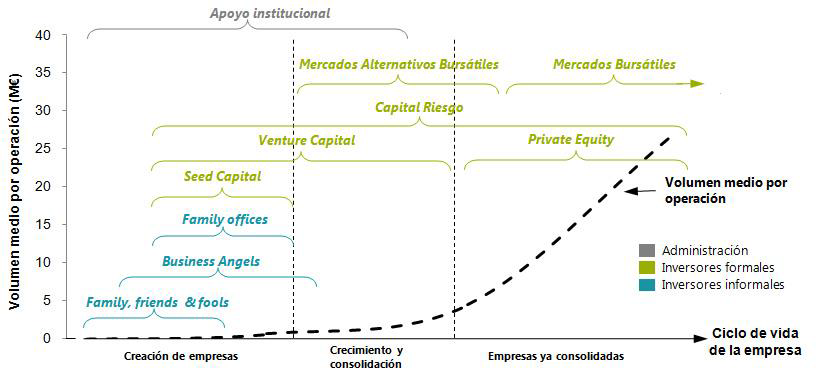
\includegraphics[width=0.8\linewidth]{figures/images/financiacion.png}
  \caption{Fuentes de financiación privada}
  \source{Pascual Parada - Creación de empresas en proyectos digitales}
  \label{fig:financiacion}
\end{figure}

\clearpage


\subsubsection{Factores socio-culturales}
Estos factores se centran en el análisis de la sociedad y el rumbo que toma en lo que se refiere a elementos como gustos, preferencias o creencias que puedan afectar al desarrollo de la actividad empresarial. Según el \acf{INE}, tanto la edad media de la población como las personas nacidas por cada 1.000 defunciones en España ha ido empeorando con el paso de los años desde el 2014 (Tabla \ref{tab:evo_edad}). Esto representa un indicador de envejecimiento progresivo del país, lo que podría ser una amenaza para la creación de la empresa.

\begin{table}[!htbp]
	\centering
	{\small
		\begin{tabular}{|c|c|c|}
\hline
\rowcolor[HTML]{343434} 
\multicolumn{3}{|c|}{\cellcolor[HTML]{343434}{\color[HTML]{FFFFFF} \textbf{Evolución indicadores población España}}}                                                                                                                                                    \\ \hline
\rowcolor[HTML]{9B9B9B} 
\multicolumn{1}{|c|}{\cellcolor[HTML]{9B9B9B}{\color[HTML]{FFFFFF} \textbf{Año}}} & \multicolumn{1}{|c|}{\cellcolor[HTML]{9B9B9B}{\color[HTML]{FFFFFF} \textbf{Edad media (años)}}} &
\multicolumn{1}{|c|}{\cellcolor[HTML]{9B9B9B}{\color[HTML]{FFFFFF} \textbf{Nacidos por cada 1.000 defunciones}}} \\ \hline
2019    & 43,39 & -          \\ \hline
2018    & 43,18 & 867,19     \\ \hline
2017    & 42,97 & 927,09     \\ \hline
2016    & 42,72 & 1.001,23   \\ \hline
2015    & 42,46 & 995,30     \\ \hline
2014    & 42,16 & 1.082,14   \\ \hline
\end{tabular}
	}
	\caption[Evolución indicadores de edad de la población en España]
	{Evolución indicadores de edad de la población en España}
	\label{tab:evo_edad}
\end{table}

Por otra parte, los cambios en la dirección de las empresas hacia el uso de los entornos \textit{cloud} favorece el cambio de mentalidad progresivamente hasta el punto en el que, en muchas ocasiones, se apuesta por entornos \textit{multicloud}, donde tres cuartos de las empresas disponen de más de una nube para impulsar su proceso de transformación digital \cite{itusermulticloud2019}. Otro ejemplo es el de AT\&T, que ha apostado por la nube de IBM  para transferir ciertas cargas de trabajo más antiguas que no pueden ser transferidas directamente a la nube, aportando una mayor capacidad en la entrega de calidad a sus clientes. 

También se debe considerar a los jóvenes tanto de la generación Y como de la Z. Estas personas se encuentran actualmente con una edad comprendida entre los 9 y los 38 años y han vivido el inicio de la digitalización y la expansión de Internet y las nuevas tecnologías. Por tanto, serán más propensas al uso de los servicios que se encuentren relacionados con ese ámbito. Siempre ha habido un crecimiento y se han implementado mejoras en la tecnología aunque, en los últimos años, la informática y todo lo que tiene que ver con ella ha sufrido unos avances importantes que han hecho que la curva de crecimiento sea exponencial. Junto a esto, también ha aumentado la tasa de población con acceso a Internet, situándose en el 86,1\% en el año 2018, donde los jóvenes de entre 16 y 24 años son los que más uso hacen (alrededor del 98\%) \cite{ineinternet}. Todo esto, junto con otros indicadores y el inevitable cambio de visión hacia el entorno \textit{cloud}, representa una oportunidad importante a la hora de llevar a cabo la creación de una empresa de este tipo.

\clearpage

\subsubsection{Factores tecnológicos}
Ya se ha hablado en el punto anterior sobre cómo las nuevas tecnologías y los entornos \textit{cloud} ayudan a las empresas en su plan de transformación digital, llegando a ser un aspecto crítico e indispensable para ello. De un tiempo a esta parte, proveedores como Amazon, Microsoft o Google han lanzado sus propias nubes en las que se ofrecen multitud de servicios que van desde los más sencillos como el almacenamiento hasta otros más complejos como la virtualización o la \acf{IA}. Algunos ejemplos de esto son visibles cuando las empresas contratan almacenamiento para alojar sus datos en servidores que pertenecen a una nube o contratan capacidad de cómputo para realizar costosas operaciones o predicciones que arrojarían datos útiles en investigaciones científicas. No obstante, por ejemplo, en el caso de la inversión en I+D, España no solo no ha mejorado sus cifras en este apartado sino que, según la \acf{FEDEA}, ha retrocedido a los valores de 2004 \cite{robertolopezvargas2019}. Por tanto, esto podría resultar una amenaza al intentar ofrecer los servicios de la empresa.

\subsubsection{Factores ecológicos}
Aunque pueda parecer que los factores ecológicos sean responsabilidad o afecten a otro tipo de industria o sector, toda actividad tiene cierto impacto, de alguna manera, en el medio ambiente. Por tanto, estos aspectos han de ser tenidos en cuenta puesto que, además, últimamente se tiene mucha conciencia en cuanto al cambio climático. De hecho, según las encuestas que realiza el \acf{CIS}, lo que se cataloga como <<problemas medioambientales>> ha ido ganando puntos en este último año en cuanto a la preocupación de los españoles. Por otra parte, también existe una legislación ambiental en España que vela por la protección de los recursos naturales. En total, suman más de 20 leyes relacionadas con el medio ambiente, aunque la principal es la Ley 21/2013, de 9 de diciembre, de evaluación ambiental, que establece el marco de competencia del Estado en cuanto a cuestiones medioambientales \cite{boemedioamb}. Dentro de esa veintena de leyes, se pueden establecer diferentes agrupaciones en cuanto a los temas que cubre cada una \cite{ceremcomunicacion2018}: 

\begin{itemize}
    \item \textbf{Aguas}. Leyes que se encargan de la protección del medio marino, contaminación y deterioro de aguas subterráneas, protección de aguas continentales y del dominio público hidráulico, vertidos de sustancias peligrosas y la protección de costas.
    
    \item \textbf{Áreas protegidas}. Se incluye el Programa de Acción Nacional de Lucha contra la Desertificación, garantías para la conservación de los hábitats naturales y temas relacionados con los Parques Nacionales y especies amenazadas.
    
    \clearpage
    
    \item \textbf{Cambio climático y energías renovables}. Se consideran las emisiones de CO2 en cuanto a las centrales eléctricas o los derechos de emisión de gases de efecto invernadero.
    
    \item \textbf{Transportes}. Regulación de aspectos de la producción de energía eléctrica en plantas solares, termoeléctricas y eólicas y aspectos relacionados con los derechos de emisión de gases de efecto invernadero.
\end{itemize}

Como se puede extraer de esta lista resumida, en España se tiene gran conciencia hacia el medio ambiente, que se ve reflejada por parte del Estado en diferentes leyes que recogen tanto derechos como deberes y obligaciones que se deben considerar a la hora de desarrollar una cierta actividad. Además, últimamente, se tiene conciencia acerca del impacto que tiene la informática en el medio ambiente, llevando a cabo proyectos como el realizado en la propia \acf{ESI}, con el fin de medir el consumo de energía de los componentes de un ordenador y su consecuente impacto en el medio ambiente \cite{auroragalisteo2019}. Esto representa el esfuerzo que se está llevando a cabo para intentar reducir la huella de carbono, donde soluciones como el \textit{cloud computing} ayudan en esta tarea, situándose como una de las tecnologías menos perjudiciales para el medio ambiente \cite{keyandcloud2018}. Por tanto, sobre todo con el cumplimiento de las leyes relativas a la emisión de gases, una empresa de nueva creación debería tener muy en cuenta estos aspectos, así como de los que se ocupan de la protección de espacios naturales o la fuente de energía eléctrica, donde la elección de un tipo de tecnología puede ser clave para el éxito de la misma.

\clearpage

\subsubsection{Factores legales}
En este último apartado del análisis PESTEL se consideran todos los aspectos que tengan que ver con la legislación vigente en el territorio de operación.

En cuanto a las leyes sobre empleo, se dispone del \acf{PAPE}, con servicios y programas de políticas activas de empleo. También se cuenta con el Real Decreto Legislativo 3/2015, de 23 de octubre, por el que se aprueba el texto refundido de la Ley de Empleo, que establece la Estrategia Española de Activación para el Empleo, los Planes a Anuales de Política de Empleo y el Sistema de Información de los Servicios Públicos de Empleo \cite{politicassepe}. 

Uno de los aspectos que se considerarían de una gran relevancia serían todos los relacionados con los datos de carácter personal, puesto que la Constitución Española recoge en su Artículo 18.4 la protección de las personas físicas en relación con el tratamiento de datos personales como un derecho fundamental. En cuanto al contexto legislativo, encontramos diferentes puntos a considerar, que se han ido desarrollando con el paso de los años \cite{aepdnormativa}:

\begin{itemize}
    \item \textbf{Directiva 95/46/CE} del Parlamento Europeo y del Consejo del 24 de octubre de 1995 (actualmente derogada), relativa a la protección de personas físicas en lo que respecta al tratamiento de datos personales y a la libre circulación.
    
    \item \textbf{Ley Orgánica 15/1999}, de 13 de diciembre, de Protección de Datos de Carácter Personal (actualmente derogada). Es decir, la \acf{LOPD}.
    
    \item \textbf{Real Decreto 1720/2007}, de 21 de diciembre, por el que se aprueba el \acf{RLOPD} (derogado).
    
    \item \textbf{Ley 11/2007}, de 22 de junio (derogada), de acceso electrónico a los Servicios Públicos, que estableció el \acs{ENS}. Este tiene como objeto determinar la política de seguridad en la utilización de medios electrónicos \cite{ens}.
    
    \item \textbf{Real Decreto 3/2010}, de 8 de enero, por el que se aprueba el \acs{ENS}.
    
    \item \textbf{Ley 40/2015}, de 1 de octubre, de Régimen Jurídico del Sector Público, recoge el \acs{ENS} en el artículo 156.
    
    \item \textbf{Real Decreto 951/2015}, de 23 de octubre, por la que se modifica el \acs{ENS} debido a la evolución del entorno regulatorio, sobre todo, de la \acs{UE}.
    
    \item \textbf{Reglamento (\acs{UE}) 2016/679 del Parlamento Europeo y del Consejo}. Es conocido como el \acf{RGPD} y, aunque entró en vigor en mayo del año 2016, es de aplicación desde el 25 de mayo de 2018, sustituyendo a la Directiva 95/46/CE que se ha mencionado anteriormente.
    
    \item \textbf{Ley Orgánica 3/2018}, de 5 de diciembre, de Protección de Datos Personales y garantía de los derechos digitales (\acs{LOPDGDD}). Modifica a la anterior \acs{LOPD} para adaptarse al \acs{RGPD}.
\end{itemize}

Por otra parte, cuando se trata con datos personales se han de tener en cuenta una serie de derechos de las personas. Aunque en la \acs{LOPD} se recogían los derechos ARCO fundamentales, con la llegada del \acs{RGPD} estos han sufrido una ligera ampliación \cite{aepdderechos}:

\begin{itemize}
    \item \textbf{Acceso}. Derecho a la obtención de la confirmación por parte del responsable del tratamiento sobre si se están tratando o no datos personales y la obtención de información.
    
    \item \textbf{Rectificación}. Derecho a la obtención de la rectificación de los datos personales inexactos.
    
    \item \textbf{Cancelación}. Derecho a la obtención de la supresión de datos cuando se den unas determinadas circunstancias.
    
    \item \textbf{Oposición}. Derecho a oposición al hecho de que los datos personales sean tratados cuando: 
    
        \begin{enumerate}
            \item Sean objeto del tratamiento basado en una misión de interés público o en el interés legítimo, incluyendo la elaboración de perfiles.
            
            \item El tratamiento tenga como finalidad la mercadotecnia directa, incluyendo también la elaboración de perfiles.
        \end{enumerate}

    \item \textbf{Portabilidad}. Derecho a la migración de datos personales de un responsable de tratamiento a otro dadas unas determinadas circunstancias.
    
    \item \textbf{Oposición (\acs{RGPD})}. Derecho a no ser objeto de una decisión basada en el tratamiento automatizado.
    
    \item \textbf{Limitación}. Derecho a la obtención de la limitación del tratamiento de los datos personales bajo unas determinadas circunstancias.
    
    \item \textbf{Información}. Derecho a la obtención de información básica por parte del responsable del tratamiento en base a dos niveles o capas de detalle.
\end{itemize}

Por último, la \acs{LOPD} establecía unos niveles de seguridad acumulativos que se aplicaban de acuerdo a la naturaleza de los datos personales. Estos niveles se pueden seguir considerando y no es necesario modificar las medidas de seguridad si ya ofrecen un nivel adecuado de seguridad. Estos niveles son los siguientes:

\begin{itemize}
    \item \textbf{Nivel básico}. Todos los datos que no sean del nivel medio o alto, con algunas excepciones. Representa el nivel por defecto y se aplica a cualquier fichero que contenga datos personales, incluyendo datos de nivel medio o alto de forma accidental o accesoria sin guardar relación con su finalidad.
    
    \clearpage
    
    \item \textbf{Nivel medio}. Datos más sensibles, como infracciones administrativas o penales, entidades de prestación de servicios de información sobre solvencia patrimonial, administraciones tributarias, entidades financieras con el fin de prestar servicios financieros, entidades gestoras de la seguridad social y mutuas o datos que permitan evaluar la personalidad o comportamiento de las personas.
    
    \item \textbf{Nivel alto}. Datos de ideología, religión o creencias, afiliación sindical, origen racial o étnico, salud, vida sexual, violencia de género y datos recabados para fines policiales sin consentimiento.
\end{itemize}

Además, es recomendable disponer de un documento de seguridad, que se trata de un documento interno que contiene el ámbito, medidas, normas y procedimientos asociados al tratamiento de datos personales del fichero. En relación a este documento existen dos posibilidades:

\begin{itemize}
    \item Documento único para todos los ficheros.
    \item Documento único para cada uno de los ficheros o ficheros relacionados.
\end{itemize}

Adicionalmente, en el caso de tratarse de datos de nivel medio o alto, se debe incluir tanto la identificación del responsable de seguridad, que será el encargado de coordinar y controlar las medidas del documento de seguridad, como recoger la obligación de realizar una auditoría bianual para verificar las medidas de seguridad.

\clearpage

\subsubsection{Conclusiones}
Una vez realizado el análisis del entorno general de operación, se considera conveniente realizar un breve resumen que contenga los aspectos más importantes de este.

En cuanto a los factores políticos, a pesar de la incertidumbre e inestabilidad política en la que se encuentra sumida España en la actualidad, algunas cifras como la \acs{TEA} han visto incrementado su valor y los expertos han valorado positivamente las iniciativas gubernamentales relativas al emprendimiento. España cuenta con un mayor número de puestos de trabajo desde la reforma laboral de hace siete años y personas relevantes como el entonces Presidente del Gobierno en funciones, Pedro Sánchez, se muestra abierto a una digitalización de la educación. Por tanto, los factores políticos podrían ser considerados como relativamente favorables.

Continuando con los económicos, la tasa de paro en España se encuentra en un descenso sostenido con las típicas fluctuaciones en los periodos críticos del año, mientras que el \acs{PIB} ha crecido en los últimos años y parece mantenerse en valores estables. Existen diferentes impuestos tales como el \acs{IRPF} o el \acs{IP} que deberían ser estudiados y sopesados; la inflación ha experimentado un crecimiento constante desde hace unos años atrás; se vive un ciclo de cierta bonanza económica con el sector de las \acs{TIC} en crecimiento y se cuenta con numerosas vías de financiación, aspecto especialmente relevante en las primeras etapas de una empresa.



A pesar de que se está experimentando un ligero envejecimiento en cuanto a la edad media de la población, cada vez se tiene más conciencia del uso de las llamadas <<nuevas tecnologías>> y el \textit{cloud}, donde el número de empresas que apuestan por una migración de sus servicios a la nube está aumentando. Considerando, además, que las personas nacidas en las últimas generaciones tienden a hacer un uso más intensivo de todos estos servicios y tecnologías, se identifica un potencial en estas que representa una oportunidad de negocio.

De la misma manera, los factores tecnológicos se ven mejorados de manera incesante gracias a las empresas ya consolidadas y la investigación que llevan a cabo en sus instalaciones de la que, posteriormente, el resto de personas se ven beneficiadas.

No obstante, los factores ecológicos y los legales son los que deberán ser tenidos muy en cuenta, sobre todo, una vez que la empresa se encuentre en el desarrollo de su actividad, ya que se tiene mucha conciencia acerca de lo que es perjudicial para el medio ambiente debido al cambio climático y de la privacidad y seguridad sobre los datos personales y privados.


\clearpage

\subsection{Análisis del entorno específico}
Una vez que se ha realizado el análisis del entorno general y se tiene una visión panorámica acerca de dónde va a operar la empresa y en qué circunstancias, se puede proceder a realizar un análisis del entorno específico, donde se valoren ciertos aspectos que afecten directamente o se encuentren relacionados con la industria objetivo. Para ello, se utilizará el análisis de las cinco fuerzas que propuso Michael Porter en 1979 y que contempla la rivalidad entre los competidores de un mismo sector, la amenaza de nuevos competidores y la de productos sustitutivos y el poder negociador de los clientes y el de los proveedores. 

Antes de realizar este análisis, conviene definir o delimitar el ámbito en el que la empresa desarrollará su actividad, puesto que está orientada a ofrecer diferentes servicios basados en \acs{DaaS} a los clientes. A su vez, esta empresa tendrá relación con otras que proporcionen servicios \acs{DaaS} a un nivel más bajo, ocupándose de todos los procedimientos de gestión que se deban realizar para proporcionar el servicio final. Una vez se tiene claro en qué posición se va encontrar la empresa, es posible comenzar el análisis del entorno específico.

\subsubsection{Rivalidad entre competidores}
Esta primera fuerza está centrada en los potenciales competidores que podría tener la empresa a la hora de desarrollar su actividad, ofreciendo el mismo tipo de producto o servicio. Cuanta mayor sea la competencia, menor será el atractivo del sector, aumentando el nivel de rivalidad entre estas empresas.

A continuación, se analizarán las diferentes propuestas que ofrece la potencial competencia, tanto las empresas con propuestas generalistas como las propuestas que se recibieron a la hora de realizar el informe <<\acf{VES}>>, del grupo \acs{TIC} de la \acs{CRUE} junto con RedIRIS \cite{rediris2015}. Este informe consideraba que las tecnologías de virtualización de escritorios tenían impacto para la gestión de los entornos informáticos, por lo que se fijó como principal objetivo aunar esfuerzos para realizar una comparación entre las diferentes propuestas existentes en el mercado que se ajustaran a las necesidades universitarias, de manera que se pueda realizar una decisión de implantación homogénea en las diferentes universidades.

\noindent\underline{\textit{\acf{NTT} Communications}}\newline
\indent \acs{NTT} \textit{Communications} es una filial de la empresa \acs{NTT} \textit{Corporation}, fundada en 1999. Esta ofrece servicios y soluciones a las empresas orientados a \textit{cloud}, \textit{data centers}, seguridad o gestión de la seguridad \cite{nttcommunications} y, según su página de información, cuenta con oficinas en 110 ciudades con centros de datos en 20 países, realiza una gran inversión en I+D y cuenta con alrededor de 10.000 clientes.

\clearpage

Uno de los servicios que ofrece se denomina \textit{Cloud-Based Desktop-as-a-Service} o \textit{Enterprise \acs{DaaS}}. Según \acs{NTT}, reduce el riesgo, incrementa la flexibilidad y es eficiente en costes para la empresa \cite{nttdaas}. Se encuentra basado en Microsoft \acs{RDS} y los recursos se encuentran alojados en los centros de datos de \acs{NTT}, por lo que los usuarios han de hacer uso de una \acs{VPN} (Arcstar UNO VPN). Se proporciona también un portal web de administración de los recursos.
 
\begin{figure}[h]
    \centering
    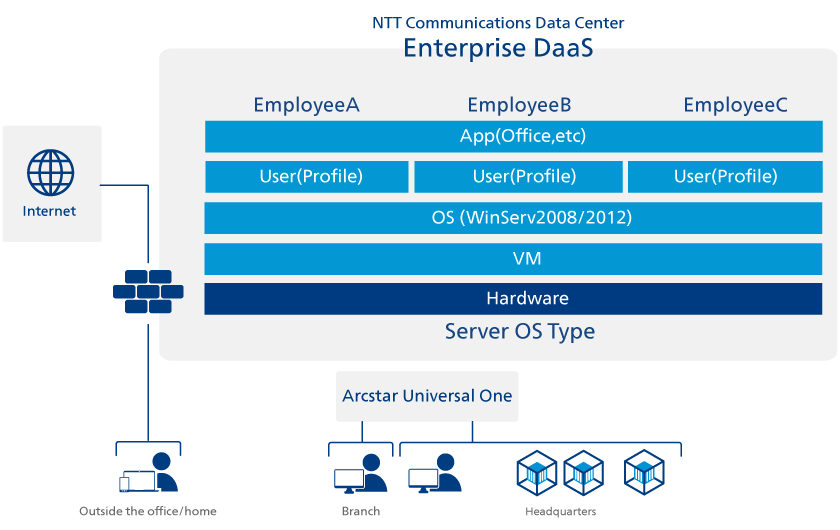
\includegraphics[width=0.8\linewidth]{figures/images/ntt_daas.png}
    \caption{\textit{\acs{NTT} Enterprise \acs{DaaS}}}
    \source{\url{https://bit.ly/2HhUENb}}
    \label{fig:ntt_daas}
\end{figure}

Como se observa en la Figura \ref{fig:ntt_daas}, los sistemas operativos que se pueden utilizar son Windows Server 2008 R2 (cuyo periodo de soporte extendido finaliza en enero de 2020 \cite{microsoftwserver2008}) o Windows Server 2012 R2, ambos en sus ediciones \textit{Datacenter}. Según las especificaciones, proporcionan Windows \acs{RDS}, con procesadores de dos núcleos, 4 \acs{GB} de memoria \acs{RAM} y 100 \acs{GB} de almacenamiento. También se incluye un \textit{help desk}, monitorización, alta redundancia, software antivirus (\textit{Virus Buster\texttrademark Corporate Edition}) y la posibilidad de aumentar o reducir la cantidad de \acs{CPU} y memoria \acs{RAM}, así como aumentar la capacidad de almacenamiento en tramos de 100 \acs{GB}. Por otra parte, según el sistema operativo que se decida escoger, se dispone de diferentes paquetes opcionales de Microsoft Office:

\begin{itemize}
    \item \textbf{Windows Server 2008 R2 Datacenter Edition 64bit}: Microsoft Office 2010 Professional, Plus o Standard.
    
    \item \textbf{Windows Server 2012 R2 Datacenter Edition 64bit}: Microsoft Office 2013 Professional, Plus o Standard.
\end{itemize}

\clearpage

\noindent\underline{\textit{Citrix Managed Desktops}}\newline
\indent Este servicio es ofrecido por parte de la empresa Citrix, que es una de las que poseen un mayor recorrido en la virtualización de aplicaciones y escritorios. Fue creada en 1989 y su oferta de valor se basa en la virtualización, redes y \textit{cloud}, principalmente, con los servicios enfocados a las empresas \cite{citrixabout}. \textit{Citrix Managed Desktops} es la solución que propone esta compañía para ofrecer servicios \acs{DaaS}, se basa en Azure y fue presentada en mayo de este año \cite{kireetivalicherla2019}. Consiste en la entrega de aplicaciones y escritorios Windows desde la nube, eliminando la administración de escritorios. Comenzó a estar disponible en el segundo cuatrimestre de 2019, aunque solo para determinados clientes de Estados Unidos, esperando su lanzamiento de manera mundial en la segunda mitad de este año. La primera versión estará basada en un escritorio de Windows Server, seguida por la versión multisesión de Windows 10 cuando esté disponible. Algunas de las características que prometen son las siguientes:

\begin{itemize}
    \item \textbf{Comprar directamente a Citrix}. Esta empresa se sitúa como una intermediaria entre el cliente y Microsoft, por lo que no será necesario tratar directamente con este.
    
    \item \textbf{Pagos por uso o mensuales}. Se podrá comprar el servicio de Citrix y los recursos de Azure de manera que se pague según el uso de estos o mediante una cuota fija mensual, aportando una mayor flexibilidad.
    
    \item \textbf{Posibilidad de asociación a un dominio}. Esto será de utilidad cuando un administrador desee provisionar un escritorio para un usuario externo. También, si la empresa dispone de este, será posible la integración de su Directorio Activo con el servicio de Citrix.
    
    \item \textbf{Soporte multiregión}. Es posible desplegar el servicio en múltiples regiones, de manera que se encuentren cercanas a la zona de operación de la empresa. Inicialmente, tendrán soporte para el este y oeste de Estados Unidos, Oeste de Europa y este de Australia, aunque se espera la adición de otras regiones en el futuro.
    
    \item \textbf{Citrix provee imágenes}. Se provee con el servicio una imagen básica de Windows con el agente <<\textit{Citrix Virtual Delivery Agent}>>, facilitando la utilización de cualquier usuario. No obstante, será posible entregar una imagen de Windows propia.
    
    \item \textbf{Construido pensando en socios externos}. Se incluirá una interfaz de usuario de gestión que permita a los socios crear servicios directamente en los escritorios gestionados por Citrix.
    
    \item \textbf{Futuro soporte de \acf{SD-WAN}}. Esto es un servicio de Citrix que ofrece la posibilidad de conectar oficinas y centros de datos a escala mundial de manera dinámica. Esto facilitará la conectividad entre los escritorios virtuales y los recursos de los que ya disponga la empresa, como el Directorio Activo.
\end{itemize}

\clearpage

\noindent\underline{Nexica \acs{DaaS}}\newline
\indent Nexica \cite{nexicaabout} es una empresa que proporciona soluciones basadas en \textit{cloud} en sus tres variantes: pública, privada o híbrida. Fue creada en 1996 y forma parte del grupo internacional Econocom. Además, cuenta con certificaciones de Cisco, trabaja con empresas como Danone, Sportium o Cáritas y sus centros de datos residen en Barcelona, Madrid y Marsella.

Uno de sus servicios es <<Nexica \acs{DaaS}>> \cite{nexicadaas}, la visión del escritorio remoto como servicio de esta empresa (Figura \ref{fig:nexica_daas}). Se trata de un servicio escalable, cuya información es almacenada en los centros de datos de Barcelona y Madrid. Al igual que sucede con la solución de Citrix, es compatible con la integración del Directorio Activo y soluciones de \acf{ERP} o \acf{CRM}. Ofrece funcionalidades y características como el panel único de provisión, que permite la creación de perfiles y escritorios y modificación de características o el soporte 24x7. Este servicio utiliza una plataforma de nube pública basada en la tecnología de \textit{VMware Horizon \acs{DaaS}} para soportar el servicio \acs{DaaS}, ofreciendo la posibilidad de realizar comunicaciones seguras a través de tecnologías como \acs{VPN}. Por último, no requiere de una inversión inicial, puesto que el método de facturación es el de pago por uso.

\begin{figure}[h]
    \centering
    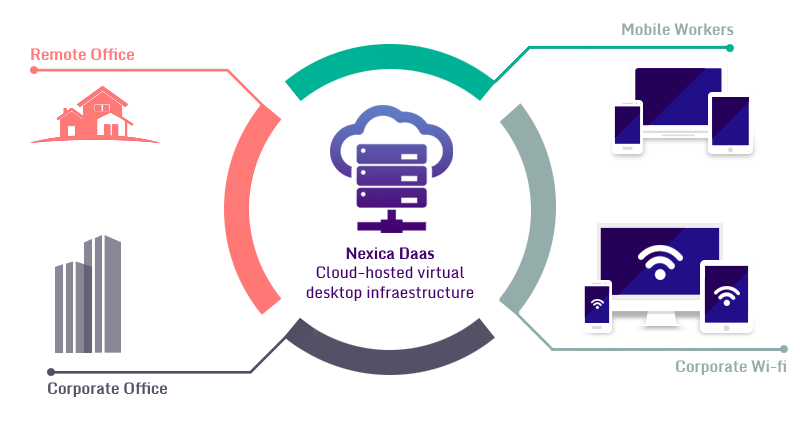
\includegraphics[width=0.8\linewidth]{figures/images/nexica_daas.png}
    \caption{Nexica \acs{DaaS}}
    \source{\url{https://www.nexica.com/sites/default/files/img/escritorios-virtuales.png}}
    \label{fig:nexica_daas}
\end{figure}

\clearpage

\noindent\underline{\textit{Flexxible Desktop}}\newline
\indent Esta es otra solución que proviene de la empresa Flexxible IT, que se creó en 2008 con un servicio \acs{DaaS} y que ofrece una plataforma \textit{cloud} para despliegues de Citrix propios y en la nube \cite{flexxibleitabout}.

Este servicio ofrece un escritorio virtual Windows, que permite a los usuarios compartir los documentos con el resto de la empresa, puesto que ofrece una solución de nube privada. Por otra parte, cuenta con facturación de pago por uso y dispone de un par de Centros de Procesamiento de Datos (\acs{CPD}) con respaldos diarios y una clasificación Tier III, lo que le aporta una disponibilidad del 99,98\% \cite{flexxiblebeneficios}. Para los administradores se proporciona un \textit{VDI Manager}, orientado a la gestión de los escritorios. Además, cuenta con unas plantillas para realizar actualizaciones o desplegar nuevos usuarios en el sistema. Por último, con este servicio se incluyen las licencias de Windows y Citrix, cuyo alojamiento de datos se encuentra en Barcelona. Existen dos modalidades que se pueden combinar en un mismo entorno \cite{flexxiblequeincluye}: 

\begin{itemize}
    \item \textbf{Premium}. Ofrece un escritorio con 1 v\acs{CPU} y 2 \acs{GB} de \acs{RAM} con 25 \acs{GB} de almacenamiento \acs{SSD} para el sistema operativo y 5 \acs{GB} para documentos y datos. Son escritorios personalizables y permiten la instalación de aplicaciones por parte del usuario.
    
    \item \textbf{Professional}. En este caso, se ofrecen 2 v\acs{CPU} y 25 \acs{GB} de \acs{RAM} con 25 \acs{GB} de almacenamiento \acs{SSD} para el sistema operativo y 5 \acs{GB} para documentos y datos. Al contrario que sucede con la modalidad \textit{premium}, son escritorios volátiles, creándose nuevos escritorios en cada conexión y conteniendo únicamente las aplicaciones que se encuentren definidas en la plantilla corporativa.
\end{itemize}

\clearpage

\noindent\underline{\textit{Dell Flexilabs}}\newline
\indent Esta es, junto con la siguiente propuesta, una de las que resultaron como las dos mejores para la implantación en entornos universitarios, según el informe \acs{VES}. Se trata de una iniciativa que lideró Joaquín Loza, de la Universidad Europea de Madrid, donde se probó y mejoró desde el año 2011. Entonces, Dell España realizó una inversión en esta solución, utilizando infraestructura de Nextel. Posee un enfoque como servicio gestionado, con experiencia en implantación en diversas universidades y una avanzada integración con la gestión académica para administrar roles y licencias. Esta propuesta ofrece tanto lo que se denomina como <<\textit{flexiLabs cloud}>> como <<\textit{flexiLabs on-site}>>. Es decir, que los servidores pueden encontrarse en la nube o en las propias instalaciones de la universidad. Algunas de las características de esta solución son las siguientes \cite{flexilabs}:

\begin{itemize}
    \item \textbf{Más de 600 aplicaciones}. Inicialmente, contaban con alrededor de 500 pero, en los últimos años, este catálogo se ha ido incrementando hasta superar las 600 aplicaciones.
    
    \item \textbf{Acceso por HTML5 o nativo}. El acceso a las aplicaciones puede realizarse de manera nativa, a través de un programa, o a través de un navegador con soporte para HTML5.
    
    \item \textbf{Distintos sistemas operativos}. Existe la posibilidad de entregar tanto escritorios basados en Linux como en Windows.
    
    \item \textbf{Orquestación y automatización}. Esto es posible gracias a los procesos integrados de automatización, por los que se obtiene la información de los estudiantes y sus asignaturas a partir de los sistemas universitarios y se les asigna las aplicaciones que pueden utilizar. Además, cuando un estudiante finaliza su vinculación con la universidad, el sistema elimina el acceso de ese estudiante a los laboratorios que contienen las aplicaciones.
    
    \item \textbf{Control del despliegue y de \acf{SLA}}. A través del catálogo online, es posible controlar y revisar el estado de las aplicaciones, publicaciones, localización, etc.
    
    \item \textbf{Tratamiento de los datos}. Los archivos de usuario se guardan de manera temporal en una carpeta, que es eliminada de manera periódica cada semana, permitiendo copiar, pegar y arrastrar entre el equipo local y el escritorio remoto. Los datos personales y credenciales son gestionados, normalmente, por la universidad, junto con el soporte a otros servicios como el Directorio Activo. Además, es posible utilizar las licencias existentes que posea la universidad para integrarlas en este servicio.
    
    \item \textbf{Informes y estadísticas de uso}. Es posible obtener reportes de uso, asignación de permisos, tipos de acceso, estadísticas de uso, etc.
\end{itemize}

\clearpage

\noindent\underline{C\textsuperscript{3}CC - \acs{UCS}}\newline
\indent Esta es una solución creada por la empresa \acf{UCS} junto con la \acf{UPM}, con la infraestructura localizada en el \acf{CeSViMa} y conectada a RedIRIS. \acs{UCS} se encuentra especializada en servicios \textit{cloud} y virtualización desde el año 2012, con integración con otras tecnologías como Netapp, Citrix y Cisco y experiencia en implantación en universidades. Según su página web \cite{c3ce}, gracias a los acuerdos que \acs{UCS} tiene con los fabricantes de \textit{thin clients} (clientes ligeros, de bajos recursos), es posible conseguir ahorros superiores al 60\% en consumo energético, junto con un ciclo de vida más largo en comparación a las soluciones tradicionales. Las características más destacadas de este servicio son:

\begin{itemize}
    \item \textbf{Ahorro}. Optimización de costes de acuerdo a la contratación de lo que se requiere.
    
    \item \textbf{Flexibilidad}. Acceso a los datos desde cualquier lugar y cuando se precise.
    
    \item \textbf{Alta disponibilidad}. Utilización de las <<últimas tecnologías de \textit{datacenter}>>.
    
    \item \textbf{Seguridad}. Toda la información se encuentra en centros de datos securizados.
\end{itemize}

\noindent\underline{Tabla comparativa}\newline
\indent A continuación, en la Tabla \ref{tab:comparativa_rivales} se expone una tabla comparativa teniendo en cuenta algunas de las características más destacadas que la mayoría de los servicios descritos comparten.

\begin{table}[hp]
	\centering
	{\small
		\begin{tabular}{p{.2\textwidth}p{.1\textwidth}p{.1\textwidth}p{.1\textwidth}p{.1\textwidth}p{.1\textwidth}p{.1\textwidth}}
    \tabheadformat
                    &
    \textbf{NTT} &
    \textbf{Citrix} &
    \textbf{Nexica} &
    \textbf{Flexxible} &
    \textbf{Dell} &
    \textbf{C3CC-UCS} \\
    \hline
    \textbf{Recursos propios} & Sí & No & Sí & Sí & Sí & Sí \\
    \hline
    \textbf{Elección de región} & No & Sí & No & No & No & No \\
    \hline
    \textbf{Tecnología de recursos} & Propia & Azure & VMware Horizon DaaS & Propia & Propia & Propia \\
    \hline
    \textbf{Portal de administración} & Sí & Sí & Sí & Sí & Catálogo & N/D \\
    \hline
    \textbf{Sistemas operativos} & Windows Server 2008/2012 & Windows Server / Windows 10 & N/D & N/D & Windows / Linux & N/D \\
    \hline
    \textbf{\textit{Help Desk}} & Sí & N/D & Sí & N/D & N/D & N/D \\
    \hline
    \textbf{Posibilidad de escalado} & Sí (por tramos) & Sí & Sí & No (Modalidades fijas) & N/D & N/D \\
    \hline
    \textbf{Enfoque} & Generalista & Generalista & Generalista & Generalista & Específico & Específico \\
    \hline
\end{tabular}
	}
	\caption[Tabla comparativa rivales]
	{Tabla comparativa rivales}
	\label{tab:comparativa_rivales}
\end{table}

\clearpage

\noindent\underline{Conclusiones}\newline
\indent Como se desprende del estudio de las diferentes alternativas entre las soluciones existentes, se observa que todas las empresas que se encuentran en este sector cuentan con cierta experiencia, lo que las convierte en unos fuertes competidores. Se considera a Citrix, con su servicio <<\textit{Citrix Managed Desktop}>> como el principal rival de la empresa que se pretende crear, debido a que su filosofía es la más cercana con la visión que se desea otorgar a dicha empresa. No obstante, no todas se encuentran enfocadas al sector educativo donde, según el estudio \acs{VES}, únicamente destacan las dos soluciones mencionadas, mientras que el resto de las propuestas son generalistas y, además, la mayoría se apoyan en servicios proporcionados por empresas externas como Citrix. Esto hace que la competencia entre empresas dedicadas al sector educativo no sea demasiado agresiva, acaparando este nicho de mercado un mayor atractivo. Además de esto, tanto las barreras de entrada como las de salida de este sector son relativamente fáciles de asumir, ya que el modelo que se intenta seguir se fundamenta en el uso de una infraestructura \textit{cloud}, permitiendo una reducción de la inversión inicial.

\clearpage


\subsubsection{Potenciales competidores}
Dentro de esta fuerza se engloban los competidores que, debido a que no han irrumpido aún en el mercado o en el sector que se está analizando actualmente, podrían realizar una competencia real en el futuro con respecto a la empresa que se desea implantar. Por lo general, la amenaza que suponen estas potenciales empresas aumentará conforme se intensifique el atractivo del sector. Por tanto, será de vital importancia posicionarse y establecerse con la mayor celeridad posible, vista la tendencia del movimiento hacia el \textit{cloud}, con el fin de comenzar a obtener una experiencia que podría ser determinante en un futuro.

Un tipo de empresas que supondría una amenaza y, por tanto, podrían postularse como potenciales competidores, serían las que se apoyaran en una nube diferente a la de, por ejemplo, Microsoft, utilizando servicios diferentes. De esta manera, los clientes que no requiriesen de una integración con los servicios de Azure podrían ver más llamativos los precios de otra empresa al ver reducidos los esfuerzos de dicha integración.

Por otra parte, si se pone el foco en las aplicaciones o programas que serían entregados, un potencial competidor que podría ser muy <<apetecible>> para los nuevos clientes (nuevas academias, empresas de reciente creación o similar) podría ser el que ofreciese una serie de paquetes de aplicaciones predefinidas. En tal caso, al estar enfocado a un cliente tan específico, puede que este, por ejemplo, aún no disponga de un conjunto de programas con los que se encuentre familiarizado para desarrollar sus tareas. Por tanto, la elección de un paquete que se ajuste a sus necesidades en una nube con los precios más competitivos y utilizando máquinas con las prestaciones mínimas, podría afianzarse como una fuerte competencia quitando un determinado segmento del mercado. Además, cabría la posibilidad de que llegasen a establecerse, a la vez, unos ciertos hábitos o dependencias en el cliente al hacer uso únicamente de las aplicaciones provistas. En este caso, considerando las universidades como potenciales clientes, se ofrecerían paquetes únicamente con las aplicaciones de las que se va a hacer uso, ahorrando costes en licencias y mantenimiento de los recursos. De esta manera, el cliente tendría que hacer frente a unos mayores costes económicos y temporales en el caso de querer cambiar de empresa.

\noindent\underline{Conclusiones}\newline
\indent El hecho de que este sector del mercado cuente con unas barreras de entrada y de salida relativamente fáciles de asumir, unido al creciente desarrollo de esta industria favorece que la amenaza de nuevos competidores con propuestas de valor diferentes y diversas sea potencialmente alta. Además de esto, el hecho de que todos los competidores puedan tener un acceso equitativo a los servicios \textit{cloud} que ofrecen los principales proveedores ratifica la consideración de alta amenaza ya mencionada. 

\clearpage


\subsubsection{Productos sustitutivos}
Otra de las fuerzas que contempla este análisis es la amenaza que puedan tener los productos sustitutivos que se podrían encontrar en el sector donde opera la empresa, facilitando el cambio a los clientes. Por tanto, el principal producto sustitutivo que se ha identificado es el conjunto de soluciones tradicionales a la hora de ofrecer escritorios o aplicaciones virtualizadas, fuera de la nube.

\noindent\underline{Instalación individual}\newline
\indent Lo que se ha denominado como <<instalación individual>> consiste en realizar una instalación de las aplicaciones y programas necesarios de manera nativa en cada uno de los terminales de usuario donde se requiera la ejecución de estos. Por tanto, cada uno dispondrá, de manera independiente, de todo lo necesario para desarrollar las tareas. Esto llevaría a un escenario donde cada terminal puede adoptar en un momento determinado un estado muy diferente a otro, como podría ser la corrupción de un archivo del que hace uso un programa específico, lo que debería repararse de manera individual, mientras que otro terminal podría encontrarse en otro estado muy diferente. Es decir, la adopción de esta solución llevaría a la empresa a una casuística difícil de controlar, ya que supondría dedicar una gran cantidad de recursos tanto a la hora de la instalación como en cuanto al mantenimiento de los diferentes terminales de usuario al presentarse potenciales estados muy diferentes entre sí.

\noindent\underline{Virtualización clásica}\newline
\indent Esta propuesta va un paso más allá con respecto a la anterior puesto que se basa en realizar una virtualización clásica, instalando un software de virtualización en cada uno de los terminales de usuario. Es decir, cada ordenador que sea utilizado por los usuarios tendrá su propia imagen base de un mismo sistema operativo. Esto requiere que dichos terminales dispongan de la suficiente potencia como para ejecutar un sistema operativo completo virtualizado, junto con las aplicaciones ejecutándose en este. Con respecto a la propuesta anterior, tiene como principal ventaja el hecho de que no es necesario instalar individualmente el software, sino que esta operación se realizaría una única vez para, posteriormente, exportar la imagen de disco e instalarla en todos los equipos. Por contra, el gran inconveniente que presenta esta solución es el de la capacidad de procesamiento que se requiere en los terminales de usuario tanto a corto como a largo plazo, aumentando el coste de los equipos.

\clearpage

\noindent\underline{\acf{RDS}}\newline
\indent Una de las soluciones un poco más avanzadas que se ha utilizado a lo largo de los años ha sido lo que se denomina como \acs{RDS} \cite{alejandroherreiz2017}. Esto consiste en la existencia de un servidor ejecutando un sistema operativo Windows Server que permite el acceso a los usuarios a una interfaz gráfica y a las aplicaciones y programas que se encuentren instalados en dicho servidor. Además, es necesario establecer una serie de roles, de manera que el servicio pueda ejecutarse (Figura \ref{fig:roles_rds}). Estos roles cumplen diferentes propósitos, como ofrecer un acceso remoto seguro, cargar las aplicaciones y ejecutarlas o virtualizar los escritorios en forma de máquinas virtuales, de manera que los usuarios no utilicen directamente el servidor. Esta solución, por tanto, es algo más dinámica y se podría ajustar a las necesidades de una empresa. No obstante, esta empresa debería realizar una inversión importante en adquirir un servidor con la suficiente potencia de computación, así como de una red que soporte todo el tráfico. Por otra parte, también se deberían tener en cuenta los gastos implícitos en los que se incurre al adoptar este tipo de solución, como el de mantenimiento, refrigeración y suministro eléctrico, siendo la capacidad de computación, además, limitada. Es decir, todos los usuarios comparten un mismo conjunto limitado de recursos; el servidor no es escalable en tiempo real por lo que, en caso de que haya una gran demanda, únicamente será posible el escalado de recursos de manera física, con el gasto económico que conlleva. Por último, habría que considerar y sopesar el tiempo de vida útil de cada uno de los componentes.

\begin{figure}[h]
    \centering
    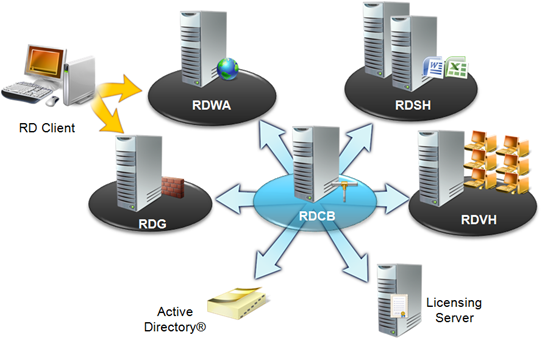
\includegraphics[width=0.6\linewidth]{figures/images/RDS_roles.png}
    \caption{Roles \acs{RDS}}
    \source{\url{https://bit.ly/2XOAr8c}}
    \label{fig:roles_rds}
\end{figure}

\noindent\underline{Conclusiones}\newline
\indent Aunque todas las opciones son viables, algunas pueden no ser factibles debido a la fuerte inversión y costes que llevan asociados. \acs{RDS} se postula como la opción con mayor peso de entre las descritas, aunque sus principales debilidades son la escalabilidad y los gastos implícitos de mantenimiento del servidor, así como la vida útil que este pueda entregar. Por tanto, el grado de sustitución del servicio que se desea implementar se considera bajo.

\subsubsection{Poder negociador de los proveedores}
De acuerdo al enfoque que se le quiere dar a la empresa, los proveedores serán aquellos que ofrezcan servicios de \acs{IaaS}, \acs{SaaS}, \acs{DaaS} o similares. Los principales proveedores de este tipo de servicios son Amazon con \acf{AWS}, Google con \textit{Compute Engine} y Microsoft con Azure.

Estas tres empresas cuentan con un respetable recorrido en este sector y todas ofrecen servicios similares. Las máquinas virtuales, el núcleo del servicio que pretende ofrecer la empresa, se ofertan con características y precios análogos en dichos proveedores. No obstante, Azure ha lanzado recientemente un servicio que puede considerarse como disruptivo con respecto a las máquinas virtuales tradicionales. Esto es lo que han denominado como \acs{WVD}, que ofrece unas funcionalidades muy concretas, como el hecho de que una misma instancia del sistema operativo pueda albergar más de un usuario al mismo tiempo, optimizando los recursos disponibles y escalando cuando sea necesario. Esto se basa en una versión especial de Windows 10 denominada <<\textit{Windows 10 Multi-Session}>>, sistema operativo que se encuentra únicamente en este servicio. Por tanto, se postula como uno de los proveedores con más peso, al proporcionar un servicio con unas funcionalidades diferenciales con respecto al resto. Por otra parte, el hecho de cambiar de un proveedor a otro puede llegar a resultar demasiado costoso en cuanto a recursos tanto materiales, como económicos o temporales, al tener que migrar todos los datos y tener que interiorizar el funcionamiento de la nueva nube.

Debido a que las soluciones tienden a ser más sencillas en cuanto al acceso, algunos de los proveedores de aplicaciones que antes debían instalarse en un ordenador de manera física, ahora tienden a ofrecer sus servicios a través de la Web. Es el caso de <<MATLAB \textit{Online}>>, un ejemplo de \acs{SaaS} del entorno de programación numérica clásico MATLAB. Por tanto, este tipo de movimientos podrían suponer un riesgo para la operación de la empresa.

Por otra parte, como se ha introducido en el párrafo anterior, se han de tener en cuenta a los proveedores no solo de servicios \textit{cloud}, sino también de las propias aplicaciones más allá de las soluciones que puedan aportar a través de servicios \acs{SaaS} propios. Sobre todo, esto se debe al tipo de aplicaciones con las que trabajan los clientes puesto que, según el proveedor de cada una, su capacidad de integración con el modelo que se pretende implantar podría presentar dificultades. Por ejemplo, si un cliente utiliza una aplicación específica y esta es la única que satisface sus necesidades, el proveedor de dicha aplicación tendrá un mayor poder de negociación sobre la empresa, puesto que el cliente no podría dar el salto a una hipotética solución ofrecida por la competencia.

\clearpage

\noindent\underline{Conclusiones}\newline
\indent Teniendo en cuenta lo anterior, el poder de negociación de los proveedores se podría considerar como relativamente alto debido a que no existe un gran número de ellos que pueda ofrecer un servicio de tan alta disponibilidad. Aunque, si los proveedores comienzan a realizar una integración hacia adelante como es el caso de MATLAB, o sus aplicaciones son muy específicas, podría suponer una amenaza para la operación de la empresa. Por otra parte, Microsoft, con \acs{WVD} ofrece un producto muy diferenciado con respecto a los demás, por lo que su poder de negociación aumenta, reduciendo al mismo tiempo la competencia.


\subsubsection{Poder negociador de los clientes}
El principal nicho de mercado que se ha identificado para la operación de la empresa es el relativo a las universidades. Es decir, la actividad y los productos de la empresa estarían enfocados al ámbito universitario. Como se ha visto anteriormente, existe cierta variedad de empresas que ofrecen los servicios de escritorios virtuales, pero la mayoría lo hacen de manera generalista, quedando pocas alternativas compatibles con los servicios que requieren las universidades. Aunque las dos propuestas que destacan poseen un cierto peso por el recorrido que tienen en cuanto a experiencia, las universidades no dispondrían de un gran catálogo de opciones para confiar la implementación de un nuevo servicio de estas dimensiones.

En cuanto a los costes que deberían asumir estas en el caso de que decidiesen cambiar de un proveedor a otro, se deberían tener en cuenta todos los servicios existentes ya implementados, como podría ser un Directorio Activo de Microsoft tanto propio como en la nube de Azure. Esto podría no ser compatible con los diferentes servicios ofrecidos por el resto de empresas y, quizá, supondría un mayor esfuerzo de integración, así como de costes asociados. Por otra parte, es conocido que el poder de negociación de los clientes aumenta cuando los productos de la industria no están diferenciados. Debido a esto, en lugar de realizar una propuesta generalista, la nueva empresa estaría orientada a ofrecer servicio únicamente a universidades, diferenciándose en gran medida del resto de propuestas y reduciendo el poder negociador de los clientes.

Por otra parte, existe la posibilidad de que las universidades realizasen una integración hacia atrás, es decir, que comiencen a crear sus propias soluciones de manera autónoma aunque, como se ha expuesto anteriormente, las alternativas existentes requerirían de un sustancial incremento de los recursos y del mantenimiento de cara a la correcta operación de los servicios. Por tanto, en principio, esto supondría un riesgo bajo en cuanto al aumento del poder negociador de los clientes.

\clearpage

Otro de los factores a tener en cuenta es la calidad percibida de la docencia en las universidades haciendo uso de ciertas herramientas. Como se comentó anteriormente en los factores socio-culturales del análisis PESTEL, se han de considerar a unos jóvenes que, cada vez, viven en una sociedad más digital. El hecho de disponer de un servicio de escritorio remoto supondría un incentivo indirecto, puesto que resultaría más atractivo para los potenciales estudiantes. Además, se podrían ofrecer las mismas posibilidades a todos los alumnos por igual, contando con la inmediatez y ubicuidad en cuanto al acceso de los recursos. Por consiguiente, estos factores se traducirían en un potencial incremento del número de matriculados, representando un estímulo para las universidades para aceptar un producto de mayor precio y/o calidad.

\noindent\underline{Conclusiones}\newline
\indent Teniendo en cuenta todo lo expuesto anteriormente en cuanto al poder negociador de los clientes, se considera que estos podrían ostentar un poder medio/bajo, al no existir una gran cantidad de alternativas especializadas, teniendo en cuenta también los demás factores discutidos a lo largo de esta sección.

\subsubsection{Tabla resumen análisis del entorno específico}
A modo de resumen del análisis del entorno específico realizado, se expone la Tabla \ref{tab:resumen_5fuerzas}, donde se encuentran las cinco fuerzas de Porter con los niveles de riesgo o amenaza correspondientes.

\begin{table}[!htbp]
	\centering
	{\small
		\begin{tabular}{|l|c|}
\hline
\rowcolor[HTML]{343434} 
\multicolumn{2}{|c|}{\cellcolor[HTML]{343434}{\color[HTML]{FFFFFF} \textbf{Análisis del entorno específico}}} \\ \hline
\rowcolor[HTML]{9B9B9B} 
\multicolumn{1}{|c|}{\cellcolor[HTML]{9B9B9B}{\color[HTML]{FFFFFF} \textbf{Fuerza}}} & {\color[HTML]{FFFFFF} \textbf{Nivel de amenaza}} \\ \hline
Rivalidad entre competidores & \cellcolor[HTML]{009901}{\color[HTML]{FFFFFF} Bajo} \\ \hline
Potenciales competidores & \cellcolor[HTML]{FE0000}{\color[HTML]{FFFFFF} Alto} \\ \hline
Productos sustitutivos & \cellcolor[HTML]{009901}{\color[HTML]{FFFFFF} Bajo} \\ \hline
Poder negociador de proveedores & \cellcolor[HTML]{FE0000}{\color[HTML]{FFFFFF} Alto} \\ \hline
Poder negociador de clientes & \cellcolor[HTML]{FFC702}Medio \\ \hline
\end{tabular}
	}
	\caption[Resumen fuerzas de Porter]
	{Resumen fuerzas de Porter}
	\label{tab:resumen_5fuerzas}
\end{table}

\clearpage

\section{Identificación de ventajas competitivas}
Una vez finalizados los estudios tanto del entorno general como del específico, esta sección del trabajo se encuentra dedicada al proceso de identificar una serie de ventajas competitivas que ayudarán a que la empresa consiga situarse en el mercado como una de las mejores opciones en cuanto a servicios \acs{DaaS}.

En primer lugar, se ha identificado que los competidores que ya se encuentran en el mercado ofrecen una propuesta generalista, donde prácticamente cualquier cliente podría contratar sus servicios y, dependiendo de este, deberían ser adaptados a sus necesidades. Por otra parte, existe una minoría de alternativas enfocadas expresamente al entorno universitario, donde una de las analizadas podría ser la más destacada del mencionado informe \acs{VES}. Por tanto, el hecho de diseñar y desarrollar una propuesta de valor específicamente orientada a un entorno universitario se podría considerar como una ventaja competitiva que podría verse potenciada con, por ejemplo, la integración de los servicios que utilicen, como el Directorio Activo en el caso de la \acf{UCLM}.

Otra de las ventajas competitivas que se han observado en el análisis del entorno específico es la capacidad de escalado. Las empresas que basan sus servicios en servidores y soluciones propias ofrecen menores posibilidades de escalado. Esto no supondría un problema para la mayoría de clientes cuyas exigencias de carga de trabajo no sean excesivamente altas, pero podría suponer un problema en el caso de las universidades, donde puede existir el escenario en el que se llevan a cabo unas tareas de computación que requieran de una gran cantidad de recursos. Además, se ha de tener en cuenta la estacionalidad de la demanda de recursos puesto que, en los periodos de vacaciones, la utilización de estos se reduciría en gran medida, derivando en una infrautilización. Disponer de recursos físicos propios que soporten un elevado número de cargas de trabajo pesadas supondría realizar una gran inversión, ya que no solo se deben tener en cuenta los propios recursos, sino también dónde van a estar ubicados, el consumo eléctrico y de refrigeración, el hecho de lidiar y alojar directamente datos de carácter personal en unas instalaciones propias o la mencionada estacionalidad. Además, estos servicios deberán contar con una disponibilidad muy alta, puesto que habrá universidades que basen su modelo de docencia en este, calificándolo como potencialmente crítico. Según un artículo en el que se tratan los costes de montar un \acs{CPD} propio \cite{cristinalopezalbarran}, se deben tener en cuenta tanto los gastos de capital como los de operación (\acf{CAPEX} y \acf{OPEX}, en inglés). En la Figura \ref{fig:costes_cpd} se pueden observar la distribución de costes a la hora de realizar una inversión en un \acs{CPD} propio.

\clearpage


\begin{figure}
    \centering
    \begin{minipage}{.5\textwidth}
        \centering
        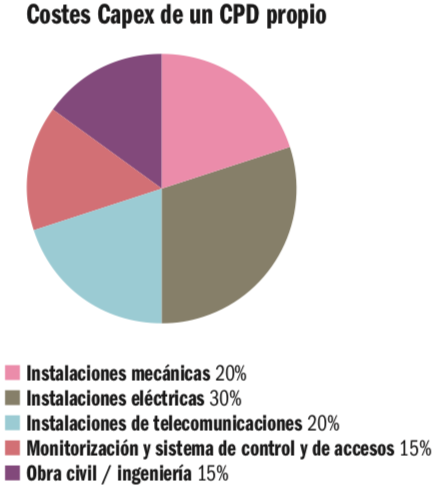
\includegraphics[width=0.75\linewidth]{figures/images/capex.png}
    \end{minipage}%
    \begin{minipage}{.5\textwidth}
        \centering
        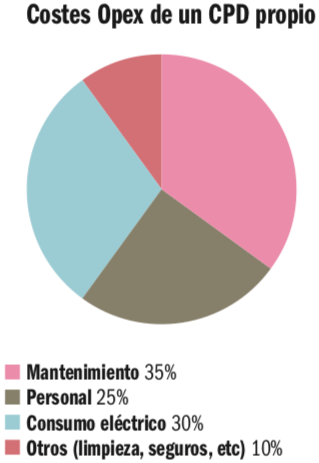
\includegraphics[width=0.55\linewidth]{figures/images/opex.png}
    \end{minipage}
    \caption{Distribución de costes \acs{CAPEX} y \acs{OPEX} de un \acs{CPD}}
    \label{fig:costes_cpd}
    \source{\url{www.datacentermarket.es}}
\end{figure}

Observando esta distribución, en el caso de externalizar los recursos, los costes \acs{CAPEX} desaparecerían, mientras que los \acs{OPEX} se verían drásticamente reducidos, pudiendo prescindir de costes como el de mantenimiento físico de los recursos o el de consumo eléctrico. Finalmente, se opta por la externalización de los recursos, que podrá dar pie a la obtención de otras ventajas competitivas debido a que se podrá destinar ese presupuesto a entregar una mayor calidad del servicio. Por tanto, contrastando los proveedores y debido al hecho de que universidades como la \acs{UCLM} hacen uso de los servicios de Microsoft, la solución que se torna como una de las más viables es la de Azure. Esta nube ofrece un servicio novedoso con respecto al resto de proveedores, con características como el escalado dinámico en función de la carga de trabajo, lo que conformará una de las ventajas competitivas más importantes.

Finalmente, en cuanto a la estrategia competitiva a seguir, partiendo de las ventajas competitivas identificadas y el análisis estratégico realizado, se decide que la que mejor se identifica con la visión es la de foco en diferenciación, en lugar de liderazgo o foco en costes. Esta estrategia tiene como objetivo centrarse en un determinado segmento de clientes de la industria que, en este caso, se tratará del segmento universitario. Por tanto, a partir de todo lo analizado y definido hasta ahora, es posible llevar a cabo el modelo de negocio de la empresa, del que se tratará en la siguiente sección del trabajo.


\clearpage


\section{Modelo de negocio}
A continuación, se describirá el modelo de negocio sobre el que se sustentará la actividad de la empresa teniendo en cuenta las conclusiones y los conocimientos adquiridos a partir del análisis estratégico anterior. Un modelo de negocio define la manera en la que la empresa crea y proporciona valor a los clientes, teniendo en cuenta los ingresos, costes y beneficios derivados de la entrega de dicho valor \cite{Teece2010BusinessInnovation}. Para ello, el modelo de negocio se apoyará en lo que se denomina como <<lienzo de modelo de negocio>> (\textit{business model canvas}, en inglés), donde se tienen en cuenta un total de nueve áreas o secciones diferentes e interrelacionadas, que se pasan a detallar en los siguientes subapartados.


\subsection{Propuesta de valor}
En este primer apartado se trata acerca de las cuestiones que tienen que ver con la entrega de valor a los clientes o consumidores finales de la empresa, de manera que se pueda satisfacer una necesidad o se proporcione un servicio o producto nuevos.

A partir del análisis estratégico, se ha identificado que la propuesta de valor que podría ofrecer la empresa es la de entregar un \textbf{servicio de virtualización de aplicaciones y escritorios} con un \textbf{alto nivel de especificación y personalización}. Es decir, no solo se podrán elegir los \textbf{aspectos básicos} de las máquinas virtuales sobre las que se ejecutarán las cargas de trabajo, sino también se podrá llevar a cabo una \textbf{selección de las aplicaciones} que se desean virtualizar, así como llevar un \textbf{control de acceso de los usuarios} a cada una de estas aplicaciones y realizar una \textbf{integración de los servicios existentes} de Microsoft con este servicio de virtualización, como pueden ser el de autenticación a través del Directorio Activo. En definitiva, otorgar un nivel de definición del servicio y asistencia superiores en comparación al resto de alternativas puesto que el foco de clientes será muy específico, personalizando dicho servicio en función de las necesidades de cada uno de ellos.

\subsection{Segmentos de clientes}
El siguiente apartado del \textit{business model canvas} hace referencia a grupos de personas o de clientes a los que va dirigida la propuesta de valor que ofrece la empresa.

Como se había apuntado en secciones anteriores de este trabajo, se había identificado que el resto de alternativas poseían un carácter más generalista, pudiendo abarcar un mayor segmento de clientes. Debido a esto, la empresa pretende centrar sus esfuerzos en desarrollar y mantener un servicio específico, con el fin de convertirse en un referente dentro de esta industria. Por tanto, el segmento de clientes que se pretende atacar será el que se encuentra relacionado con el ámbito de la docencia y, más concretamente, a las universidades, donde el número de empresas que ofrecen este tipo de servicios es relativamente escaso.

\subsection{Canales}
Una vez se tiene clara la propuesta de valor y el segmento de clientes al que se pretende dirigir, esta sección del modelo de negocio aborda cómo y por qué vías se ofrece dicha propuesta de valor al cliente.

La empresa concentrará sus esfuerzos en una publicidad no invasiva, aunque eficaz. Es decir, se comunicará a las universidades los servicios que ofrece la empresa a través de los contactos que estas proporcionen, tratando directamente con el departamento de tecnologías o similar. Además, la empresa comenzará disponiendo de una sede local con vistas a expansión a diversos puntos estratégicos de la geografía, donde también será posible informar a los nuevos clientes mediante una cita concertada. De la misma manera, se dispondrá de una página web donde estos clientes encontrarán toda la información que requieran, de manera que pueda servir de ayuda en la toma de decisiones.

\subsection{Relaciones con el cliente}
Las relaciones que mantenga la empresa con el cliente y viceversa son un factor que debe ser tenido muy en consideración, puesto que la experiencia que el cliente obtenga durante el tiempo que se mantenga la relación entre ambos será determinante para que este continúe confiando en la empresa y sus servicios.

No obstante, una vez que se haya logrado una conversión del cliente, también se pretende que este tenga la posibilidad de contactar con la empresa de una manera más ágil por otros medios como el correo electrónico tradicional, un \textit{help desk} para resolver las posibles incidencias o peticiones críticas que puedan ocurrir en el servicio, asistencia vía telefónica o a través de un \textit{chatbot} en la página web de la empresa que pueda ayudar tanto a nuevos clientes a encontrar información con una mayor rapidez como a los ya existentes a encontrar una solución a sus necesidades. Se apuesta también por una relación directa, donde las sedes tomarán una mayor relevancia, siendo un lugar donde cliente y empresa tengan la oportunidad de hablar cara a cara a la hora de proporcionar la información que se precise en cada momento, así como para tratar temas delicados.

\subsection{Actividades clave}
Como su nombre indica, esta sección se encontrará dedicada a exponer las actividades que poseen el mayor peso dentro de la actividad de la empresa y que permiten la entrega de la propuesta de valor al cliente.

La empresa tendrá la publicidad y el marketing como una de las actividades clave, puesto que su segmento de clientes es muy específico, por lo que se deberá profundizar en este para obtener una cartera de clientes de la que se puedan obtener beneficios. Además, el hecho de personalizar el servicio para cada uno de los clientes será otra actividad clave, puesto que es uno de los pilares en los que se apoya la propuesta de valor.

\subsection{Recursos clave}
El presente apartado del modelo de negocio se encuentra relacionado con los elementos más importantes que permiten que dicho modelo funcione y se desarrolle en la manera que se busca.

Uno de los principales recursos clave es intangible y debe ser potenciado y maximizado. Se trata de la sensación que percibe el cliente de que está obteniendo un servicio único, de manera que se pueda afianzar la relación con la empresa y sea duradera, creando una imagen de marca sólida, consistente y atractiva. Otro de los recursos clave será la capacidad tecnológica, esencial en la integración del servicio de la empresa con los recursos ya existentes de Microsoft de los que disponga el cliente, de manera que la migración de datos sea mínima o nula proporcionando, de cierto modo, un ecosistema en el que todo se encuentre relacionado. Finalmente, un recurso clave esencial serán las sedes, con las que se pretende tener presencia en lugares estratégicos y que permitirán el hecho de dar a conocer a la empresa, así como aumentar la notoriedad en dichos lugares.

\subsection{Socios clave}
La mayoría de las empresas, además de disponer de unos recursos clave, suelen recurrir a unos determinados socios con los que se establecen determinadas relaciones que asisten en la operación de la empresa. Por tanto, este tipo de relaciones toman una cierta relevancia cuando se trata de entregar la propuesta de valor al cliente.

Indudablemente, si la empresa desea proporcionar unos servicios \textit{cloud} en la nube de Azure, el principal socio clave será Microsoft, encargado de proporcionar toda la tecnología y el acceso a la misma. Además, proporcionaría servicios adicionales que asistan en la comunicación con los clientes mediante herramientas como Skype Empresarial o para la coordinación de equipos con soluciones como Microsoft Teams. Esta decisión ha sido tomada en consideración con el análisis del sector específico y las ventajas competitivas, donde se ha identificado a Microsoft y su servicio \acs{WVD} como el que ofrece un mayor potencial gracias a funcionalidades innovadoras e integración con otros servicios.

No obstante, la empresa no dispondrá de Microsoft como único socio clave, sino que también entrarán en juego los proveedores de otras aplicaciones que requieran los clientes y con los que se pueda trabajar para permitir su integración en la solución de Microsoft y poder mejorar así el servicio final entregado. De esta manera, a su vez, los propios clientes podrían llegar a convertirse en un un socio clave más, fruto de la relación mantenida a lo largo del tiempo puesto que, si la empresa cumple con los acuerdos establecidos y las expectativas y se trabaja de manera conjunta en la mejora del servicio, la empresa podría ser recomendada a futuros clientes, aumentando su cartera.

\subsection{Estructura de costes}
Esta sección se encuentra dedicada a la definición de la estructura de costes, es decir, los gastos a los que la empresa debe hacer frente durante su tiempo de actividad.

Considerando la actividad de la empresa y el apartado anterior relativo a los socios clave, uno de los principales costes a asumir será el de la infraestructura tecnológica que, si bien no se dispone de ella físicamente, su uso conlleva un coste asociado que dependerá de Microsoft. Otro coste a tener en cuenta será el correspondiente al mantenimiento de las diferentes sedes de las que se ha hablado con anterioridad. Estos costes, al no tener unos servidores propios para dar servicio, se verán reducidos considerablemente, aunque deberá hacerse frente a una determinada inversión inicial en la primera sede con la compra o alquiler de unas oficinas, así como de sus servicios básicos. Además, se deberá realizar una campaña de marketing que, en su fase inicial tendrá un carácter más agresivo, para dar a conocer los servicios que ofrece la empresa y los beneficios derivados de su uso. Una vez que la empresa se encuentre en una situación estable, los principales costes serán los de los trabajadores, así como el mantenimiento de las instalaciones.

\subsection{Fuentes de ingresos}
Finalmente, la última sección o apartado del lienzo de modelo de negocio se encuentra dedicada a exponer cómo y de qué fuentes una empresa obtiene determinados ingresos.

Principalmente, la empresa propuesta obtendrá sus ingresos gracias a los servicios que preste y que añadan valor al servicio ofrecido por Microsoft, apoyándose en Azure, su plataforma \textit{cloud}. Es decir, los ingresos serán fruto de los esfuerzos de la integración de los servicios y datos existentes obtenidos de cada cliente para llevar a cabo una parametrización, personalización y puesta en marcha a partir del servicio de Azure, satisfaciendo las necesidades de dichos clientes de manera individual e incorporando mejoras propias de valor añadido que faciliten tareas como la gestión de usuarios.





\clearpage

\section{Implementación de un servicio \acs{DaaS} en \acs{WVD}}
A continuación, se expondrán los pasos seguidos para llevar a cabo la creación del servicio \acs{DaaS} en la plataforma \textit{cloud} de Azure. Del mismo modo, se detallarán las tareas de programación que se deberán realizar para el desarrollo de una aplicación con el objetivo de facilitar la gestión de usuarios de dicho servicio.

\subsection{Creación del servicio de \acs{WVD}}
La primera tarea que ha de efectuarse para desplegar el servicio de \acs{WVD} es su creación en la nube de Azure. Para ello, se han seguido los pasos descritos en la documentación oficial \cite{microsofttutowvd}, que deben ser ejecutados con una cuenta de administrador de la suscripción de Azure. Para ello, el primer paso que se debe realizar es el de crear un inquilino (\textit{tenant}), es decir, un conjunto de uno o más \textit{host pools}. Cada uno de estos \textit{host pools} serán los que alberguen las máquinas virtuales que ofrecerán tanto aplicaciones remotas como escritorios remotos completos, según la configuración que se desee otorgar a cada usuario. Para ello, se deben cumplir algunos requisitos previos, entre los que destaca disponer de una suscripción a Azure y disponer del identificador del Directorio Activo de Azure (\textit{Azure Active Directory ID}). El Directorio Activo de Azure permite disponer de manera centralizada del total de los usuarios, clasificados por grupos y con permisos para cada uno de ellos. Por tanto, se hace más sencilla la gestión de los mismos en servicios como el que se desea implementar.

El primer paso que se debe realizar es proporcionar los permisos del Directorio Activo requeridos por el servicio de \acs{WVD}. Para ello, se debe acceder a la página de consentimiento \url{https://rdweb.wvd.microsoft.com} y otorgar los permisos de \textit{server app} y \textit{client app} al identificador del Directorio Activo de Azure (Figura \ref{fig:consentAAD}).

\begin{figure}[h]
  \centering
  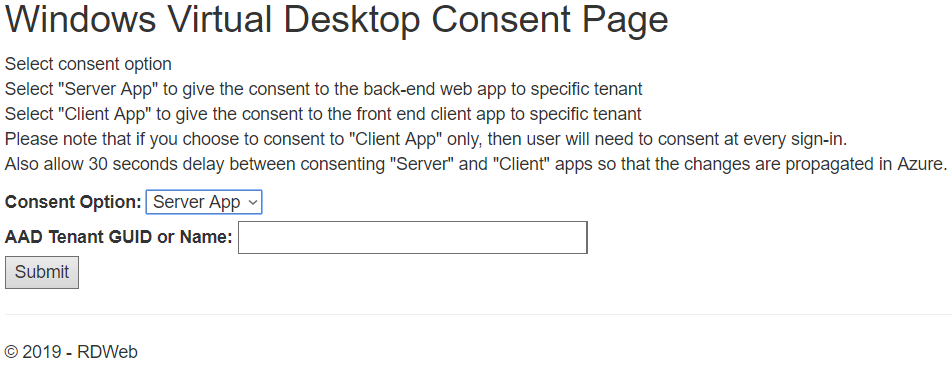
\includegraphics[width=0.8\linewidth]{figures/images/consentAAD.PNG}
  \caption{Página de consentimiento de \acs{WVD}}
  \label{fig:consentAAD}
\end{figure}

\clearpage

Una vez se han proporcionado los permisos requeridos al servicio de \acs{WVD}, se debe asignar el rol <<\textit{TenantCreator}>> a un usuario que se encuentre en el Directorio Activo permitiendo a dicho usuario crear nuevos inquilinos de \acs{WVD}. Para ello, se deberá acceder al portal de Azure con la cuenta de administrador (\url{https://portal.azure.com/}) y, dentro de la categoría <<servicios>> en <<\textit{enterprise applications}>>, seleccionar <<\textit{Windows Virtual Desktop}>>. Una vez dentro del servicio, en <<\textit{Users and groups}>>, añadir el usuario que se quiere que tenga los privilegios de creación de inquilinos.

Para los siguientes pasos, se debe disponer tanto del identificador de directorio (\textit{directory ID}) como del identificador de la suscripción (\textit{Azure subscription ID}). Para este propósito, se deberá buscar <<\textit{Azure active directory}>> y <<\textit{subscriptions}>> en la barra de búsqueda para copiar los valores requeridos de cada uno de los elementos.

El servicio de \acs{WVD} se encuentra en fase de beta pública (\textit{public preview}) y, según Microsoft, se espera que sea lanzado a finales del 2019, por lo que la mayoría de los procedimientos se realizarán a través de la consola de PowerShell. Teniendo esto en cuenta, es necesaria la instalación e importación del módulo de \acs{WVD} en PowerShell utilizando los siguientes comandos:

\begin{console}
    Install-Module -Name Microsoft.RDInfra.RDPowerShell
\end{console} %$

\begin{console}
    Import-Module -Name Microsoft.RDInfra.RDPowerShell
\end{console} %$

A continuación, se debe iniciar sesión en \acs{WVD} utilizando la cuenta de usuario que se ha establecido anteriormente para la creación de nuevos inquilinos:

\begin{console}
    Add-RdsAccount -DeploymentUrl "https://rdbroker.wvd.microsoft.com"
\end{console} %$

\begin{console}
    New-RdsTenant -Name <TenantName> -AadTenantId <DirectoryID> -AzureSubscriptionId <SubscriptionID>
\end{console} %$

\begin{console}
    New-RdsTenant -Name Contoso -AadTenantId 00000000-1111-2222-3333-444444444444 -AzureSubscriptionId 55555555-6666-7777-8888-999999999999
\end{console} %$

Posteriormente, se debe crear lo que se denomina como \textit{service principal} en el Directorio Activo de Azure y asignarle un rol dentro de \acs{WVD}, que será el que despliegue el \textit{marketplace} para crear \textit{host pools}. Para crear un \textit{service principal} y asignar roles, se debe instalar el siguiente módulo de PowerShell:

\begin{console}
    Install-Module AzureAD
\end{console} %$

A continuación, se puede proceder a la creación del \textit{service principal} en el Directorio Activo de Azure:

\begin{console}
    Import-Module AzureAD
    $aadContext = Connect-AzureAD
    $svcPrincipal = New-AzureADApplication -AvailableToOtherTenants $true -DisplayName "Windows Virtual Desktop Svc Principal"
    $svcPrincipalCreds = New-AzureADApplicationPasswordCredential -ObjectId $svcPrincipal.ObjectId
\end{console} %$

Una vez que se ha completado la creación del \textit{service principal}, es posible su utilización para acceder al servicio de \acs{WVD}. Para asignar un rol a este usuario, se ejecutan los siguientes comandos:

\begin{console}
    Add-RdsAccount -DeploymentUrl "https://rdbroker.wvd.microsoft.com"
    New-RdsRoleAssignment -RoleDefinitionName "RDS Owner" -ApplicationId $svcPrincipal.AppId -TenantName $myTenantName
\end{console} %$

Por último, si todo ha sido creado correctamente, se podrá acceder con el usuario \textit{service principal} para, posteriormente, crear \textit{host pools} y crear y asignar grupos de aplicaciones a los diferentes usuarios que se encuentren dentro del Directorio Activo de Azure:

\begin{console}
    $creds = New-Object System.Management.Automation.PSCredential($svcPrincipal.AppId, (ConvertTo-SecureString $svcPrincipalCreds.Value -AsPlainText -Force))
    Add-RdsAccount -DeploymentUrl "https://rdbroker.wvd.microsoft.com" -Credential $creds -ServicePrincipal -AadTenantId $aadContext.TenantId.Guid
\end{console} %$

\clearpage

\subsection{Creación de un \textit{host pool} en Azure}
Una vez que se dispone del inquilino (\textit{tenant}) de \acs{WVD} en Azure, es necesario crear un \textit{host pool}, que principalmente será un conjunto de máquinas virtuales con las mismas características, disponibles según la demanda que haya en un determinado momento \cite{microsofttutohostpool}. Además, a cada uno de ellos se le podrá asignar un grupo de aplicaciones, de manera que los usuarios que tengan acceso a ese \textit{host pool} solo puedan ejecutar las aplicaciones para las que se les ha dado permiso.

\subsubsection{Parámetros básicos}
Para realizar esta tarea, se deberá acudir al portal de Azure (\url{www.portal.azure.com}) y crear un nuevo recurso desde el menú que aparece en la barra vertical situada a la izquierda para, posteriormente, seleccionar el resultado <<\textit{
Windows Virtual Desktop - Provision a host pool}>>. A continuación, se debe introducir una serie de parámetros para la configuración:

\begin{itemize}
    \item \textbf{\textit{Hostpool name}}. Nombre que recibirá ese \textit{host pool}.
    
    \item \textbf{\textit{Desktop type}}. En esta configuración se dispone de dos opciones.
    
        \begin{itemize}
            \item \textbf{\textit{Pooled}}. Esta opción será de utilidad cuando se desea que una misma máquina virtual pueda ser utilizada por diferentes usuarios. Es decir, que una máquina virtual pueda albergar simultáneamente a varios usuarios a la vez. Por tanto, con esta configuración se ganará eficiencia y se reducirán costes, puesto que los mismos recursos serán utilizados por un grupo de usuarios.
            
            \item \textbf{\textit{Personal}}. En este caso, a diferencia del anterior, cada usuario dispone de su propia máquina virtual. Esto es útil cuando las máquinas han de ser específicamente asignadas a determinados usuarios y, además, estos usuarios pueden ser administradores locales de esas máquinas, cosa que no sería posible con la configuración anterior.
        \end{itemize}
        
    \item \textbf{\textit{Default desktop users}}. Aquí se escribirán las direcciones de correo que se encuentren en el Directorio Activo de los usuarios que se desea que tengan acceso a este \textit{host pool}. En el futuro, según Microsoft, se podrán agregar grupos de usuarios. No obstante, esto puede ser cambiado a través de la línea de comandos de PowerShell, como se verá más adelante.
    
    \item \textbf{\textit{Subscription}}. La suscripción de Azure de la que ya se disponga.
    
    \item \textbf{\textit{Resource group}}. Cada uno de los \textit{host pools} requiere de un grupo de recursos que pueda utilizar, entre ellos se encuentra una interfaz de red y un soporte de almacenamiento. Se deberá seleccionar uno que se encuentre vacío o crear uno nuevo.
    
    \clearpage
    
    \item \textbf{\textit{Location}}. Localización donde se crearán los recursos necesarios. En esta ocasión, se seleccionará \textit{West Europe}, puesto que la suscripción de Azure se encuentra ligada a esta. Es conveniente, por otra parte, seleccionar la ubicación más cercana con el fin de reducir tiempos de carga y transmisión de datos.
\end{itemize}

\subsubsection{Configuración de las máquinas virtuales}
Una vez rellenados estos campos y completada la primera parte de la creación del \textit{host pool}, se procede a elegir la configuración de las máquinas virtuales. Se puede elegir el perfil de uso (\textit{light}, \textit{medium}, \textit{heavy} o \textit{custom}) y el número total de usuarios para obtener esa recomendación (Figura \ref{fig:asistente_mv}).

\begin{figure}[h]
  \centering
  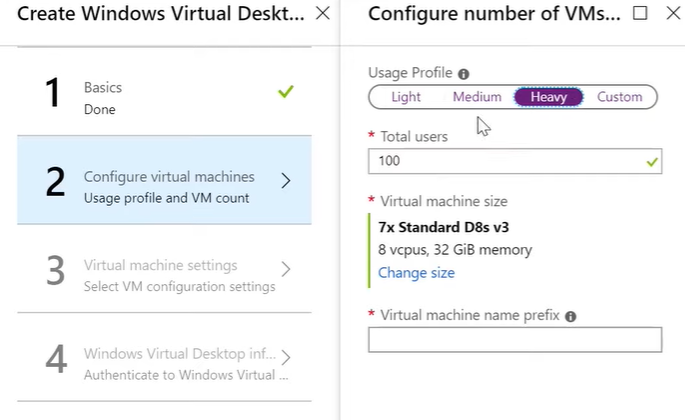
\includegraphics[width=0.6\linewidth]{figures/images/asistente_mv.PNG}
  \caption{Asistente de configuración de máquinas virtuales}
  \label{fig:asistente_mv}
\end{figure}

A pesar de que se dispone de un sencillo asistente que ayudará a la hora de tomar la decisión, es posible elegir el tipo de máquinas virtuales del \textit{host pool} de manera manual en el catálogo que se encuentra disponible (Figura \ref{fig:tipos_mv}).

\begin{figure}[h]
  \centering
  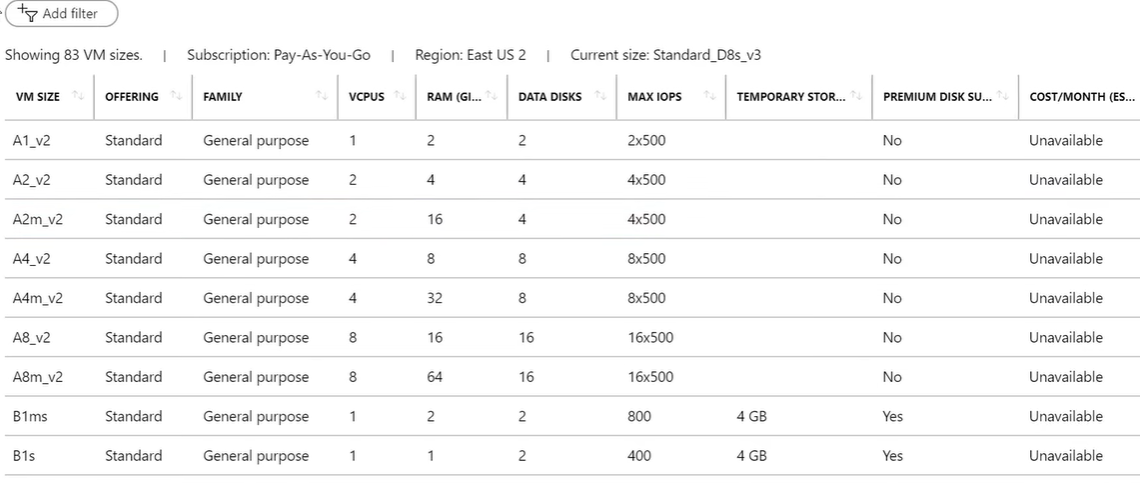
\includegraphics[width=0.8\linewidth]{figures/images/tipos_mv.PNG}
  \caption{Catálogo de configuraciones de máquinas virtuales}
  \label{fig:tipos_mv}
\end{figure}

Por último, se le deberá asignar un prefijo, que será el que utilicen todas las máquinas virtuales dentro de ese \textit{host pool}. Es decir, si se establece el prefijo como <<vm-wdPrueba>>, todas las máquinas virtuales y los correspondientes recursos utilizarán ese prefijo, añadiendo un número como sufijo para identificarlas.

\subsubsection{Parámetros de las máquinas virtuales}
A continuación, se deben especificar los parámetros más específicos que atañen a las máquinas virtuales. El primero de ellos es escoger si se desea utilizar una imagen de sistema operativo propia que se ha de subir a Azure o una que se encuentre disponible entre las que ofrece Microsoft, que son las siguientes:

\begin{itemize}
    \item \textbf{\textit{Windows 10 Enterprise multi-session with Office 365 ProPlus}}. Esta imagen está preparada con una versión de Windows 10 especial, puesto que admite varias sesiones de manera simultánea. Por tanto, hace posible que un grupo de usuarios se conecten y hagan uso de una misma máquina virtual.
    
    \item \textbf{\textit{Windows 10 Enterprise multi-session}}. Imagen idéntica a la anterior, exceptuando que no contiene el paquete de Microsoft Office 365 ProPlus.
    
    \item \textbf{\textit{Windows Server 2016 Datacenter}}. Esta imagen representa un sistema operativo más clásico, orientado a servidores con un enfoque tradicional.
\end{itemize}

En \textbf{\textit{disk type}} es posible seleccionar el tipo de disco duro que usarán estas máquinas virtuales entre dos opciones disponibles: discos duros mecánicos tradicionales o unidades de estado sólido. A continuación, en los campos \textbf{\textit{AD domain join UPN}}, \textbf{\textit{Admin Password}} y \textbf{\textit{Confirm Password}} se deberán introducir las credenciales que se han creado previamente para el \acf{UPN}. Por último, se debe especificar una \acf{OU} y una red virtual que utilizarán las máquinas de este \textit{host pool}.

Finalmente, en el último paso aparecen unos campos que se deberán rellenar con el nombre que se desea asignar al \textit{host pool}, así como las credenciales del \acs{UPN}. Una vez terminado el proceso, comenzará el despliegue del servicio con la configuración proporcionada. Cuando este haya finalizado, se habrán creado una serie de recursos que deberían aparecer de una manera similar a los que se muestran en la Figura \ref{fig:recursos_azure}.

\begin{figure}[h]
  \centering
  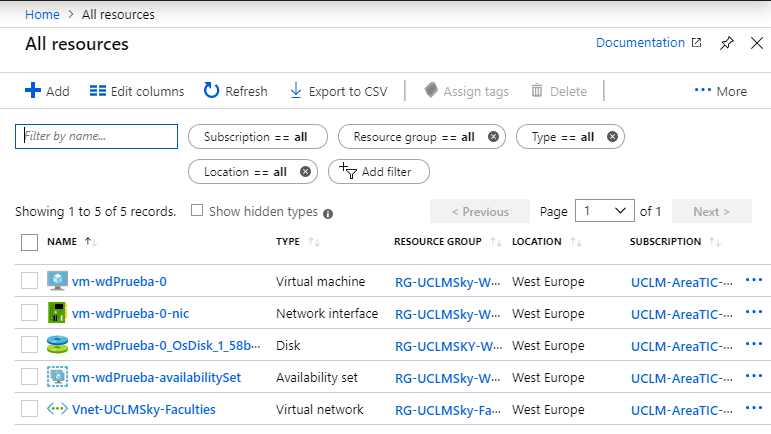
\includegraphics[width=0.8\linewidth]{figures/images/recursos_azure.PNG}
  \caption{Recursos creados en Azure}
  \label{fig:recursos_azure}
\end{figure}

Uno de los recursos es el relativo a la propia máquina virtual; otro representa la interfaz de red a la que se encuentra conectada al recurso de la red virtual y un recurso que simboliza el disco duro de la máquina. Finalmente, se encuentra un recurso del tipo <<\textit{availability set}>>, que es una abstracción que se encarga de agrupar y aislar todos los recursos pertenecientes a una máquina del resto de máquinas o servicios desplegados, de manera que se pueda aumentar la disponibilidad, asegurando que si un grupo de recursos cae, otros podrán continuar ofreciendo el servicio. Por último, para levantar el servicio, únicamente faltaría arrancar la máquina virtual. Para ello, se deberá acceder al recurso del tipo <<\textit{virtual machine}>> y presionar el botón \textit{start} (Figura \ref{fig:iniciar_mv}) para que, tras unos instantes, el servicio se encuentre disponible y sea accesible por todos los usuarios a los que se les haya otorgado el acceso en la configuración anterior.

\begin{figure}[h]
  \centering
  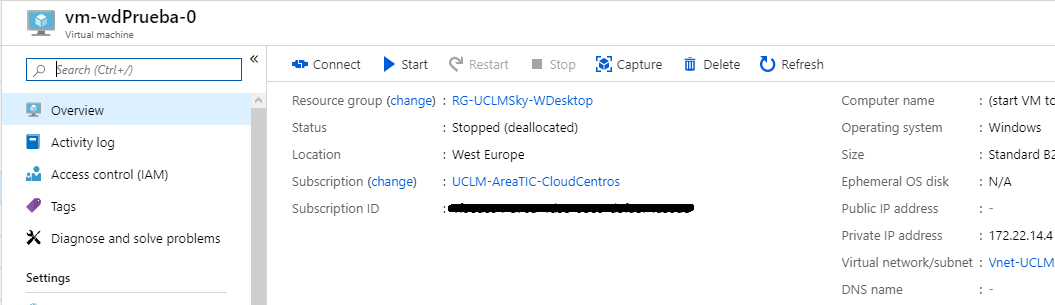
\includegraphics[width=0.9\linewidth]{figures/images/iniciar_mv.PNG}
  \caption{Iniciar máquina virtual}
  \label{fig:iniciar_mv}
\end{figure}

\clearpage

\subsection{Desarrollo de una solución de gestión de usuarios para \acs{WVD}}
Una vez que se dispone de todos los recursos necesarios para ejecutar y proporcionar el servicio, se deben realizar tareas como la creación de grupos de aplicaciones y la asignación de los diferentes usuarios a los grupos de aplicaciones correspondientes, de manera que puedan hacer uso únicamente las aplicaciones que estos requieran. Actualmente, Microsoft ofrece una única manera de realizar estas tareas de administración, y es mediante comandos en la consola de PowerShell. En la documentación oficial, incluso se llega a mencionar que se deberían programar bucles en PowerShell en el caso de que se desee añadir más de un usuario a la vez a un grupo de aplicaciones, de manera que el mismo comando se ejecute varias veces para otorgar acceso a todos las direcciones necesarias. Por tanto, se ha tomado la decisión de desarrollar una solución propia con el fin de asistir en la realización de estas tareas de gestión y administración del servicio, haciendo que dichas tareas resulten más fáciles e intuitivas de realizar a través de una interfaz gráfica. Esta interfaz fue diseñada en un paso anterior al comienzo de la tarea de programación, realizando unos bocetos que se encuentran en el Anexo \ref{anx:bocetos}, utilizando para ello la aplicación <<\textit{Balsamiq Mockups}>>. También se tuvieron en cuenta las acciones que el usuario podría llevar a cabo mediante la utilización de esta aplicación, realizando el diagrama de casos de uso que puede consultarse en el Anexo \ref{anx:diagrama_cdu}.

\subsubsection{Ventana de conexión a Azure}
Lo primero que se ha de realizar para establecer una conexión con el servicio de \acs{WVD} creado es iniciar sesión en Azure. Para llevar a cabo esta tarea se ofrece al usuario una ventana desde la que se podrá iniciar o cerrar sesión, en el caso de que ya se encontrara iniciada (Figura \ref{fig:main_conex}).

\begin{figure}[h]
  \centering
  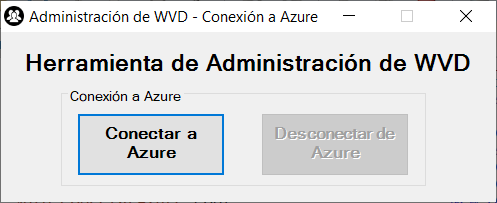
\includegraphics[width=0.7\linewidth]{figures/images/script/main_conex.PNG}
  \caption{Ventana de conexión a Azure}
  \label{fig:main_conex}
\end{figure}

\clearpage

Una vez se pulse sobre el botón de <<Conectar a Azure>>, se abrirá una ventana nueva para ingresar el correo electrónico de la universidad y rellenar con el usuario y contraseña los campos en la identificación de la organización propia que, en este caso, sería la \acs{UCLM} (Figuras \ref{fig:inicio_microsoft} y \ref{fig:inicio_uclm}).

\begin{figure}
    \centering
    \begin{minipage}{.5\textwidth}
        \centering
        
\includegraphics[width=0.8\linewidth]{figures/images/script/inicio_microsoft.PNG}
        \caption{Inicio de sesión en Microsoft}
        \label{fig:inicio_microsoft}
    \end{minipage}%
    \begin{minipage}{.5\textwidth}
        \centering
        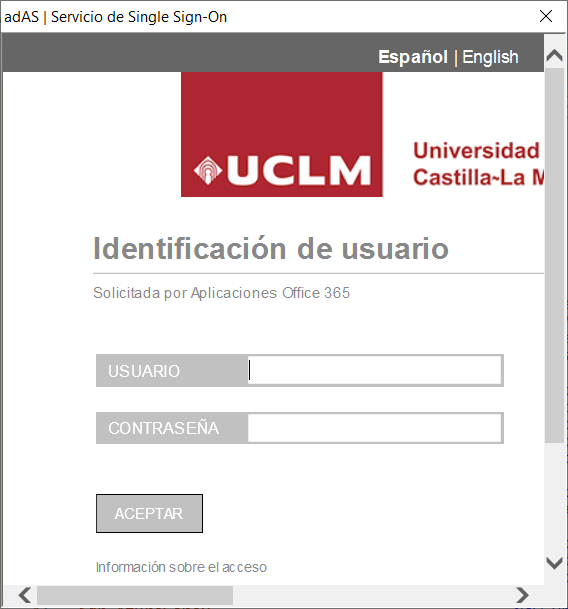
\includegraphics[width=0.8\linewidth]{figures/images/script/inicio_uclm.PNG}
        \caption{Inicio de sesión en la \acs{UCLM}}
        \label{fig:inicio_uclm}
    \end{minipage}
\end{figure}

Tanto si el inicio de sesión ha sido satisfactorio o ha fallado debido a unas credenciales mal introducidas o ha habido un problema durante el proceso, se avisará al usuario con una ventana. Suponiendo que dicha autenticación se haya producido correctamente, la ventana representada en la Figura \ref{fig:main_conex} se expandirá para que el usuario pueda introducir las credenciales del servicio de \acs{WVD} que se le proporcionaron en su creación.

\begin{figure}[h]
  \centering
  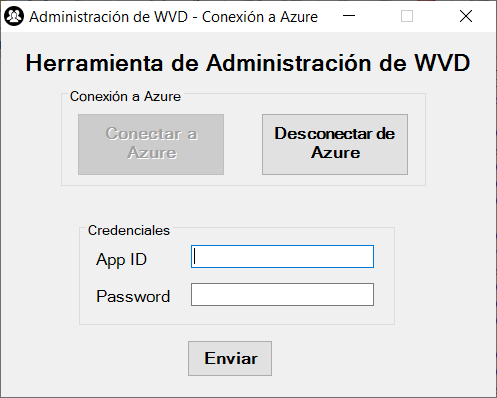
\includegraphics[width=0.6\linewidth]{figures/images/script/main_expand.PNG}
  \caption{Ventana de conexión al servicio de \acs{WVD}}
  \label{fig:main_expand}
\end{figure}

\subsubsection{Ventana de menú principal}

Una vez que el usuario se haya autenticado en el servicio correspondiente de \acs{WVD}, accederá a lo que se ha denominado como <<ventana de menú principal>> (Figura \ref{fig:menu_ppal}), desde donde se podrán realizar dos tareas diferenciadas: consultar los \textit{hostpools} que se encuentran creados y disponibles en dicho servicio y llevar a cabo una gestión de los grupos de aplicaciones de cada uno de dichos \textit{hostpools}.

\begin{figure}[h]
  \centering
  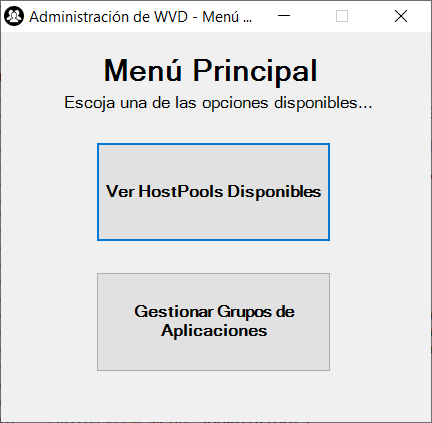
\includegraphics[width=0.6\linewidth]{figures/images/script/menu_ppal.PNG}
  \caption{Ventana de menú principal}
  \label{fig:menu_ppal}
\end{figure}

\clearpage

\noindent\underline{Ver \textit{hostpools} disponibles}\newline
\indent Desde esta ventana, el usuario dispondrá de una lista desplegable desde la que podrá ver todos los \textit{hostpools} que se encuentran disponibles en el servicio. Además, seleccionando alguno de ellos, se podrán visualizar sus propiedades y parámetros con los que fue configurado (Figura \ref{fig:info_hostpools}).

\begin{figure}[h]
  \centering
  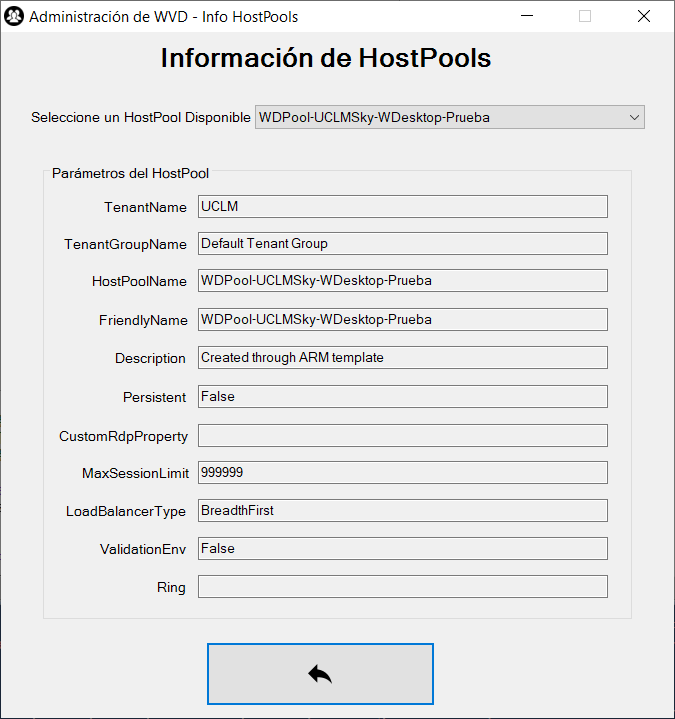
\includegraphics[width=0.7\linewidth]{figures/images/script/info_hostpools.PNG}
  \caption{Ventana de información de \textit{hostpools}}
  \label{fig:info_hostpools}
\end{figure}

\clearpage

\noindent\underline{Gestionar grupos de aplicaciones}\newline
\indent Como se ha indicado anteriormente, desde el menú principal será posible acceder también a la gestión de los grupos de aplicaciones de cada uno de los \textit{hostpools} mediante la ventana de gestión de grupos (Figura \ref{fig:ventana_gestion}). De manera similar al procedimiento para visualizar la información de los \textit{hostpools}, en este caso se deberá seleccionar uno de los disponibles a partir de la lista desplegable que se encuentra en la parte superior de la ventana. De esta manera, la lista de grupos de aplicaciones se rellenará con los que se encuentren creados en ese momento. Se permitirá al usuario, seleccionando un grupo de aplicaciones, ver sus parámetros, aplicaciones disponibles y usuarios con acceso haciendo doble clic sobre la lista o pulsando el botón correspondiente, así como la edición de usuarios y aplicaciones pulsando sobre el botón de editar parámetros.

\begin{figure}[h]
  \centering
  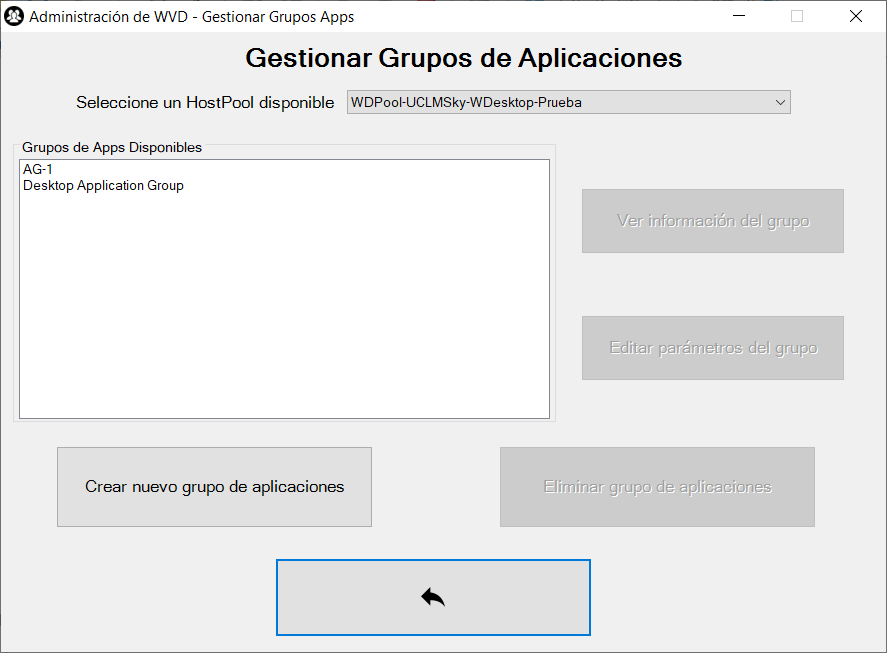
\includegraphics[width=0.7\linewidth]{figures/images/script/ventana_gestion.PNG}
  \caption{Ventana de gestión de grupos}
  \label{fig:ventana_gestion}
\end{figure}

La Figura \ref{fig:ventana_infogrupo} representa lo que vería el usuario al hacer doble clic sobre un grupo de aplicaciones de la lista o al pulsar sobre el botón para ver la información del grupo seleccionado. En esta ventana, se pueden visualizar los parámetros con los que fue creado el grupo en la parte izquierda, mientras que la parte derecha se encuentra reservada a las listas de aplicaciones y usuarios de ese grupo de aplicaciones, que se encuentran deshabilitadas para su edición. En el caso particular de que el grupo de aplicaciones sea de tipo <<\textit{desktop}>>, no se mostrará ninguna aplicación debido a que este tipo de grupo ofrece a los usuarios el escritorio virtual completo, por lo que no tiene restricciones en este ámbito. Debido a este motivo, en lugar de aplicaciones, se mostrará un único mensaje advirtiendo que este tipo de grupo no es compatible con la selección de aplicaciones (Figura \ref{fig:ventana_infogrupoDesktop}).

\begin{figure}[h]
  \centering
  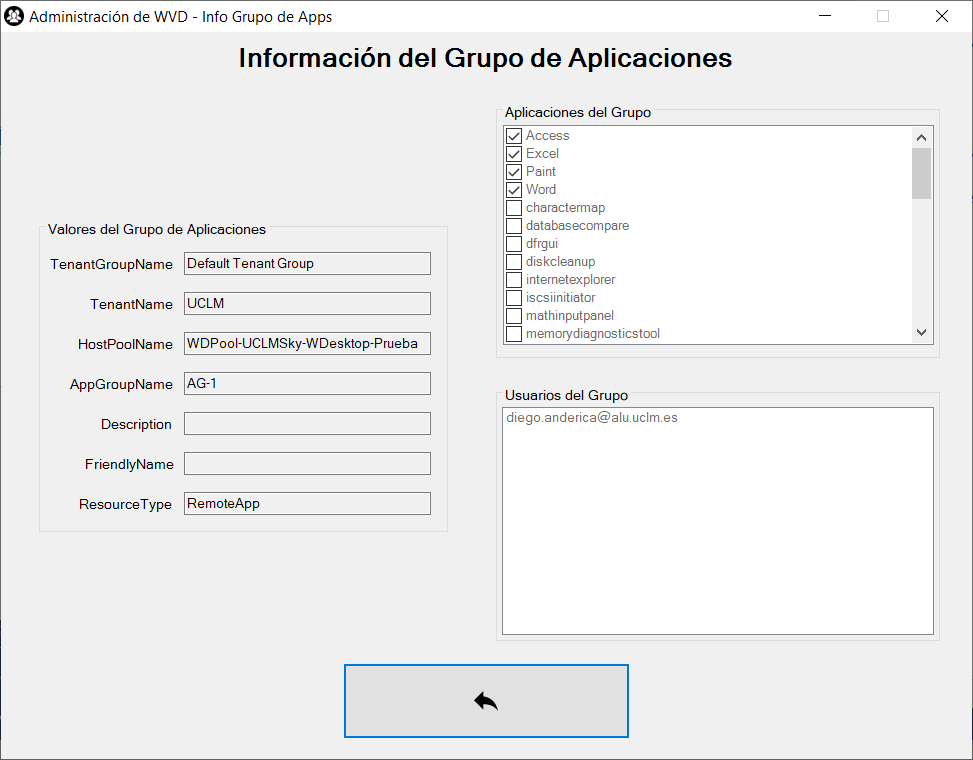
\includegraphics[width=0.7\linewidth]{figures/images/script/ventana_infogrupo.PNG}
  \caption{Ventana de información de grupo}
  \label{fig:ventana_infogrupo}
\end{figure}

\begin{figure}[h]
  \centering
  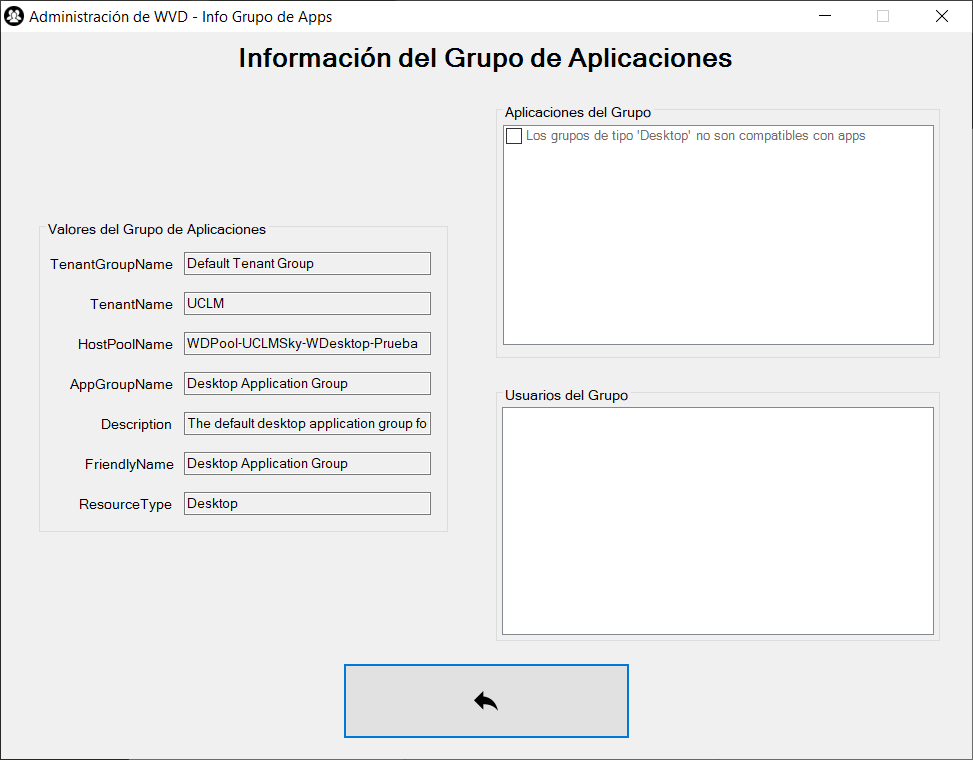
\includegraphics[width=0.7\linewidth]{figures/images/script/ventana_infogrupoDesktop.PNG}
  \caption{Ventana de información de grupo (\textit{ResourceType Desktop})}
  \label{fig:ventana_infogrupoDesktop}
\end{figure}

\clearpage

En el caso de que el usuario desee editar tanto la lista de aplicaciones disponibles como otorgar o revocar el acceso al grupo a los diferentes usuarios, deberá seleccionar un grupo de la lista y pulsar sobre el botón de editar parámetros. De esta manera, se abrirá una ventana similar a la anterior pero, en esta ocasión, las listas de aplicaciones y usuarios se encontrarán habilitadas y se mostrarán botones adicionales en la parte derecha (Figura \ref{fig:ventana_editargrupo}). En cuanto a las aplicaciones, el usuario podrá seleccionar las que desee de entre las disponibles y pulsar sobre el botón <<guardar cambios de aplicaciones>> para que la nueva selección quede establecida. En cuanto a los usuarios con acceso, se pondrán a disposición del usuario tres botones con los que llevar a cabo esta gestión: comenzando por el superior, este permite añadir una o varias direcciones de correo para otorgarles permiso de acceso al grupo, introduciéndolas manualmente; el botón central posibilita utilizar un archivo \acs{CSV} con todos los usuarios a los que se desea otorgar acceso, sustituyendo a los existentes; finalmente, el último se utiliza para revocar el acceso al usuario seleccionado.

\begin{figure}[h]
  \centering
  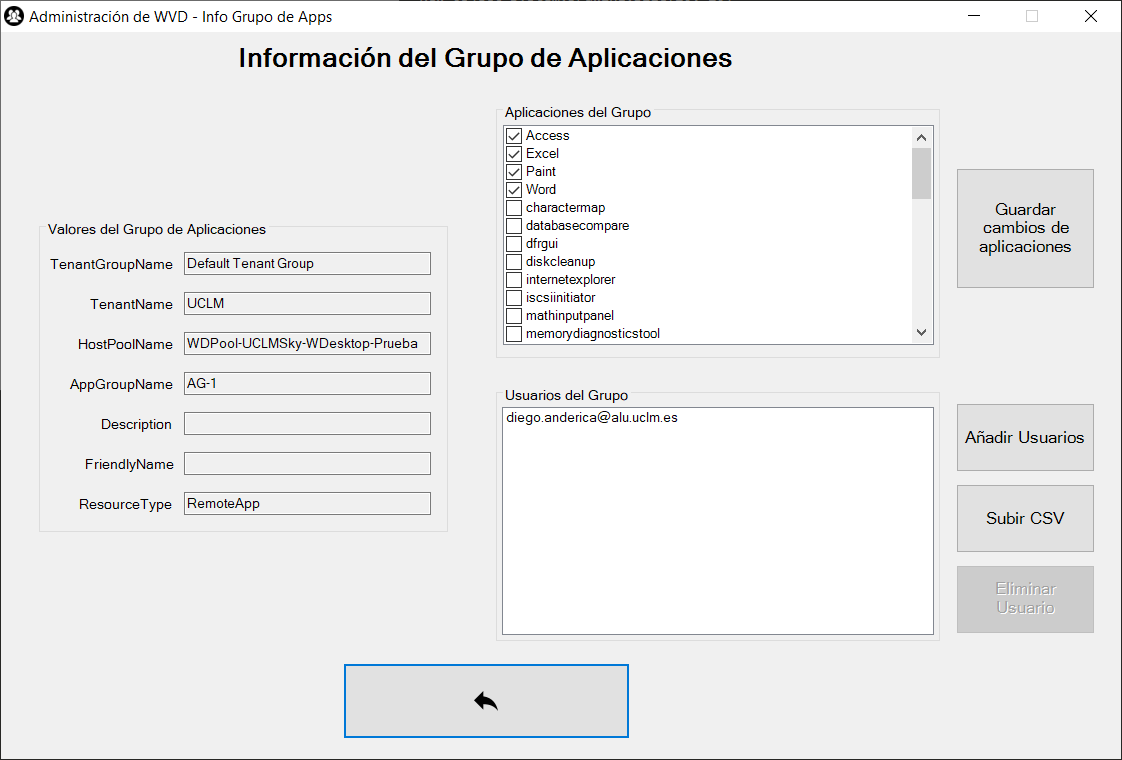
\includegraphics[width=0.7\linewidth]{figures/images/script/ventana_editargrupo.PNG}
  \caption{Ventana de edición de grupo}
  \label{fig:ventana_editargrupo}
\end{figure}

\clearpage

Finalizando con las funcionalidades de este script, como se mostraba en la Figura \ref{fig:ventana_gestion}, se dispone de otros dos últimos botones para la creación y eliminación de los grupos de aplicaciones. En el caso de que se desee crear un nuevo grupo, se abrirá una nueva ventana para introducir los parámetros básicos para su creación (Figura \ref{fig:ventana_creargrupo}). En cuanto al tipo de recursos, se podrá elegir entre <<\textit{RemoteApp}>> y <<\textit{Desktop}>>, donde el primero representa un grupo de aplicaciones como tal, mientras que el segundo establece un grupo donde se ofrece el escritorio completo. Por último, para eliminar un grupo, bastará con seleccionarlo en la lista y pulsar sobre el botón de <<eliminar grupo de aplicaciones>>.

\begin{figure}[h]
  \centering
  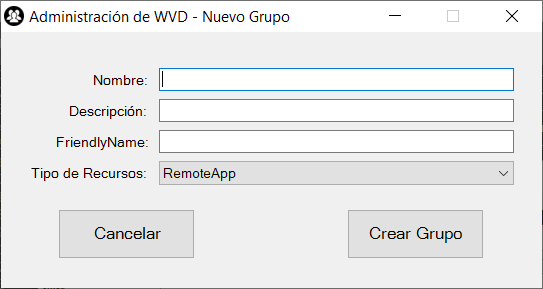
\includegraphics[width=0.6\linewidth]{figures/images/script/ventana_creargrupo.PNG}
  \caption{Ventana de creación de grupo}
  \label{fig:ventana_creargrupo}
\end{figure}

\clearpage

\subsection{Desarrollo de diferentes casos de uso}
Con el objetivo de comprobar la viabilidad del servicio creado y documentar los pasos necesarios para la entrega de diferentes configuraciones de este en función de las necesidades, se han planteado y desarrollado dos diferentes casos de uso. El primero de ellos se encuentra enfocado a los equipos que podrían ubicarse en las aulas de libre uso de una biblioteca de un campus universitario. Por otra parte, el segundo será más específico, puesto que estará destinado a ofrecer las herramientas necesarias para el seguimiento por parte de los alumnos de la asignatura <<Fundamentos de Programación I>> del Grado en Ingeniería Informática impartido en el Campus de Ciudad Real. A pesar de que buena parte de los pasos a realizar tienen carácter común para cualquier despliegue que se realice, se detallarán las puntualizaciones necesarias para cada uno de los casos de uso.

\subsubsection{Creación de la imagen a utilizar}
Es posible seleccionar un sistema operativo sobre el que se han instalado las herramientas necesarias de manera personalizada a la hora de crear un nuevo \textit{hostpool}, puesto que este servicio permite utilizar imágenes propias, como se ha indicado anteriormente. Para ello, se debe crear una máquina virtual en Azure, independiente del servicio de \acs{WVD}. Por tanto, con el objetivo de tener un orden en cuanto a los recursos en Azure, se ha creado un nuevo grupo de recursos que se ha denominado como <<RG-UCLMSky-WDesktop-PlantillaW10>>. Dentro de este grupo sería donde se crearían todas las máquinas virtuales necesarias para poder prestar los diferentes tipos de servicio, de acuerdo con las necesidades de los clientes. Una vez que dicho grupo ha sido creado, se procede a añadir un nuevo recurso, buscando <<Windows 10>> en el \textit{marketplace} de Azure y seleccionando <<Microsoft Windows 10 + Office 365 ProPlus>>, en alguna de sus dos versiones disponibles actualmente (Figura \ref{fig:seleccion_w10}).

\begin{figure}[h]
  \centering
  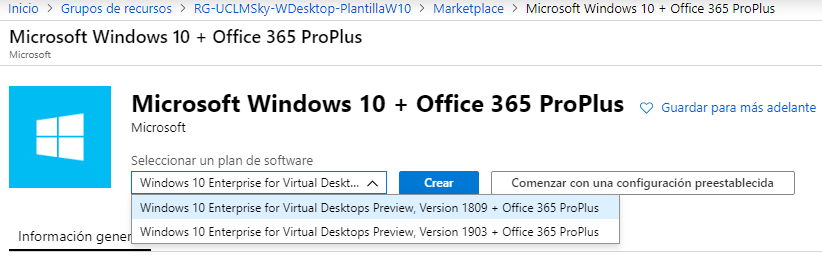
\includegraphics[width=0.8\linewidth]{figures/images/casos_uso/MVW10.PNG}
  \caption{Imágenes de Windows 10}
  \label{fig:seleccion_w10}
\end{figure}

Esto comenzará un proceso para la creación de una máquina virtual con la imagen de Windows deseada, donde será necesario indicar parámetros como el nombre de esta, los recursos de \acs{CPU} y memoria o si se desea o no utilizar discos administrados. En cuanto a este último punto, se ha decidido no utilizar discos administrados, utilizando una cuenta de almacenamiento y obteniendo algunas ventajas como la de descargar el disco duro completo para su virtualización en un equipo local llegado el momento.

\subsubsection{Aprovisionamiento de la máquina}
Una vez que se ha creado una máquina virtual, será momento de conectarse a esta para instalar las herramientas necesarias. Para cada uno de los casos de uso citados anteriormente se ha preguntado a los diferentes involucrados, obteniendo una lista por cada uno de ellos:

\begin{itemize}
    \item \textbf{Aulas de libre uso}. Involucrado: Manuel Díaz-Marta Puentes (técnico de sistemas y redes en el \acs{CTIC} de la \acs{UCLM}).
    
        \begin{itemize}
            \item Adobe Acrobat Reader.
            \item Navegador Google Chrome.
            \item Microsoft Office Professional Plus 2016.
            \item EndNote Plug-Ins.
            \item ResearchSoft Direct Export Helper.
        \end{itemize}
        
    \item \textbf{Fundamentos de Programación I}. Involucrados: Jesús Serrano Guerrero, María del Carmen Lacave Rodero y Ester del Castillo Herrera (docentes de la asignatura en la \acs{ESI} de Ciudad Real).
    
        \begin{itemize}
            \item Adobe Acrobat Reader.
            \item \acf{JDK}.
            \item NetBeans.
            \item Eclipse.
        \end{itemize}
\end{itemize}

Como se puede observar, en el caso de las aulas de libre uso, se requieren herramientas destinadas a la visualización y edición de documentos, así como de un navegador de Internet y unos \textit{plugins} cuya labor se centra en la citación de referencias bibliográficas. Por otra parte, en el caso de la asignatura de Fundamentos de Programación I, se requieren herramientas relacionadas con el aprendizaje del lenguaje de programación Java, como son su kit de desarrollo o los programas NetBeans y Eclipse, para la edición de código. Lamentablemente, debido a la forma de instalación por defecto de Eclipse, este no es compatible con la manera de proceder de la herramienta <<\textit{sysprep}>>, de la que se hablará más adelante. Finalmente, al igual que sucede con las aulas de libre uso, también se hace necesario un lector de archivos \acs{PDF} para que los alumnos puedan seguir en sus equipos el material que ha sido elaborado por el personal docente.

Una vez finalizado este paso, se ha creado un nuevo grupo de recursos para almacenar una copia de seguridad de las máquinas en Azure. Este procedimiento será recomendable puesto que, una vez que se ejecute la herramienta <<\textit{sysprep}>>, las máquinas se apagarán y no podrán ser accedidas de nuevo debido al propio funcionamiento de dicha herramienta.

\clearpage

\subsubsection{Realizar \textit{sysprep} a la máquina}
Este paso será de vital importancia a la hora de crear un nuevo \textit{hostpool} utilizando el sistema operativo sobre el que se han instalado las herramientas anteriores. La utilidad denominada <<sysprep>> se encarga, en cierto modo, de limpiar Windows y de apagarlo, de manera que la próxima vez que se inicie se pida al usuario toda la información inicial. Esto dejaría el disco duro en un estado similar al que se encuentra el de un ordenador proporcionado por un proveedor con Windows 10 preinstalado justo antes de su primer arranque.

Dicha herramienta se incluye en Windows 10 y es posible encontrarla en la siguiente ruta: C:\textbackslash Windows\textbackslash System32\textbackslash Sysprep\textbackslash sysprep.exe y deberá ejecutarse con las opciones indicadas en la Figura \ref{fig:conf_sysprep}.

\begin{figure}[h]
  \centering
  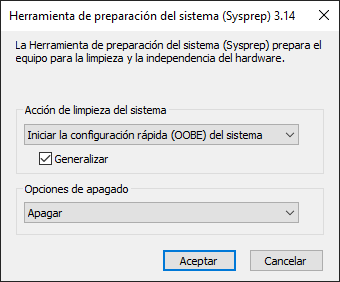
\includegraphics[width=0.5\linewidth]{figures/images/casos_uso/sysprep.PNG}
  \caption{Configuración sysprep}
  \label{fig:conf_sysprep}
\end{figure}

Una vez que el proceso haya finalizado, la máquina virtual se habrá apagado pero no desasignado. Es decir, aunque efectivamente se encuentra apagada, los recursos que Azure le había asignado continúan bloqueados, por lo que será necesario detener la máquina desde el panel de Azure. En caso contrario, continuaría contando para la facturación.

A continuación, será necesario obtener la dirección donde se encuentra la imagen del disco \acs{VHD} para indicarlo en el proceso de creación de un nuevo \textit{hostpool}. Para ello, dentro de la máquina virtual, en el menú lateral, se debe acudir al apartado <<discos>> y acceder al disco que estaba asignado a dicha máquina (Figura \ref{fig:menudiscos}).

\clearpage

\begin{figure}[h]
  \centering
  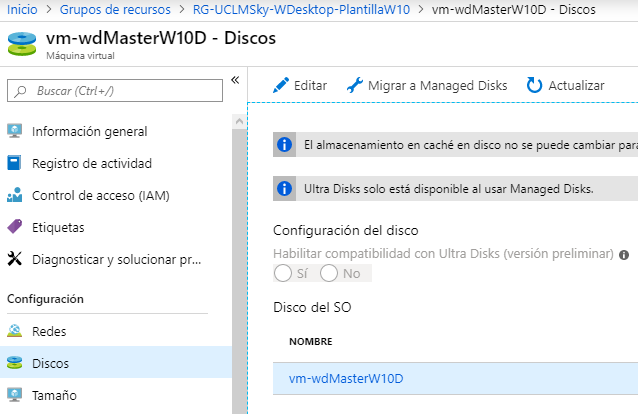
\includegraphics[width=0.5\linewidth]{figures/images/casos_uso/discosVM.PNG}
  \caption{Menú <<discos>> de la máquina virtual}
  \label{fig:menudiscos}
\end{figure}

Una vez dentro del disco, se deberá copiar el campo <<\acs{URI} de \acs{VHD}>>, puesto que será requerido para especificar dónde se encuentra la imagen que se desea utilizar para un nuevo \textit{hostpool} (Figura \ref{fig:uri_vhd}).

\begin{figure}[h]
  \centering
  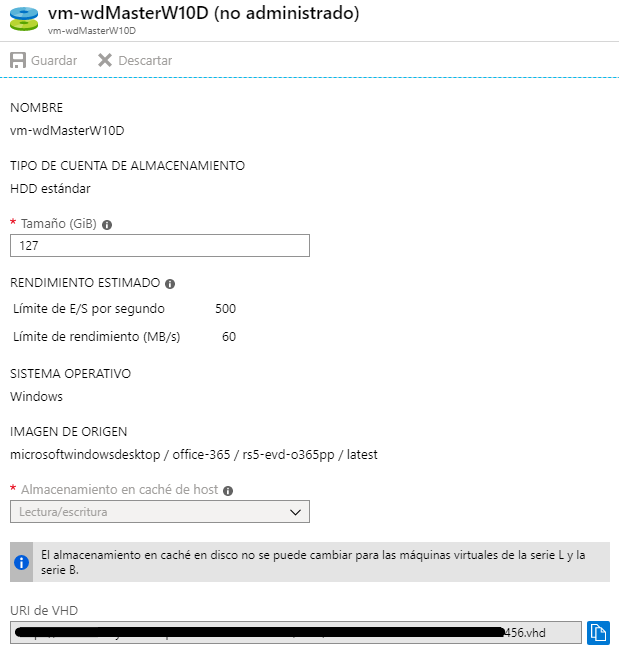
\includegraphics[width=0.7\linewidth]{figures/images/casos_uso/uri_vhd.PNG}
  \caption{\acs{URI} de \acs{VHD}}
  \label{fig:uri_vhd}
\end{figure}

Finalmente, se podrá realizar el aprovisionamiento de un nuevo \textit{hostpool} como se ha indicado en un apartado anterior de este capítulo con la salvedad de que, en este caso, no se utilizará una imagen proporcionada por Microsoft, sino que se utilizará la imagen personalizada, pegando en el campo correspondiente la dirección \acs{URI} deseada.

\subsubsection{Creación de grupos de aplicaciones}
Una vez que se han creado ambos \textit{hostpools}, se han establecido unos grupos de aplicaciones y se ha dado acceso a un usuario de la Universidad, a modo de prueba, a cada uno de dichos grupos. A continuación, se explicarán los pasos realizados para llevar a cabo estas tareas.

\noindent\underline{Aulas de libre uso}\newline
\indent En el caso de las aulas de libre uso, se selecciona el \textit{hostpool} correspondiente en la aplicación y se crea un nuevo grupo de aplicaciones del tipo <<\textit{RemoteApp}>>, puesto que se desea entregar aplicaciones virtualizadas en lugar del escritorio completo (Figura \ref{fig:cg_alu}).

\begin{figure}[h]
  \centering
  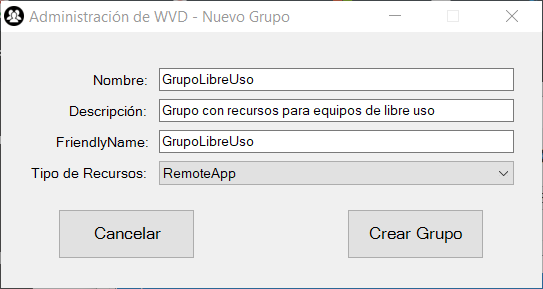
\includegraphics[width=0.5\linewidth]{figures/images/casos_uso/creacion_grupo_alu.PNG}
  \caption{Creación del grupo para aulas de libre uso}
  \label{fig:cg_alu}
\end{figure}

Cuando la aplicación ha terminado de crear el nuevo grupo de aplicaciones, se editan los parámetros de este para seleccionar las aplicaciones que se desean entregar, así como a los usuarios a los que se desea dar acceso a dicho grupo (Figura \ref{fig:params_alu}).

\begin{figure}[h]
  \centering
  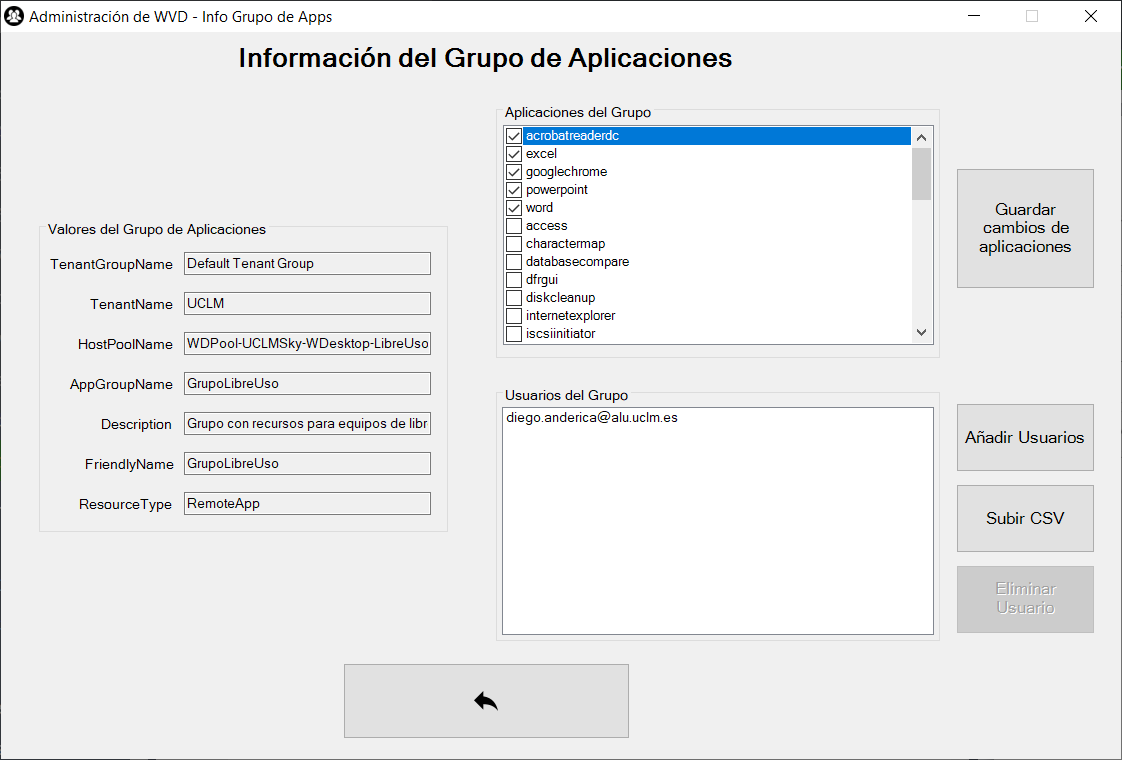
\includegraphics[width=0.8\linewidth]{figures/images/casos_uso/params_alu.PNG}
  \caption{Parámetros para aulas de libre uso}
  \label{fig:params_alu}
\end{figure}

\clearpage

\noindent\underline{Fundamentos de Programación I}\newline
\indent De igual manera, para el caso de la asignatura de Fundamentos de Programación I, se crea un nuevo grupo de aplicaciones del tipo <<\textit{RemoteApp}>> en el \textit{hostpool} destinado para este caso de uso (Figura \ref{fig:cg_ffppi}).

\begin{figure}[h]
  \centering
  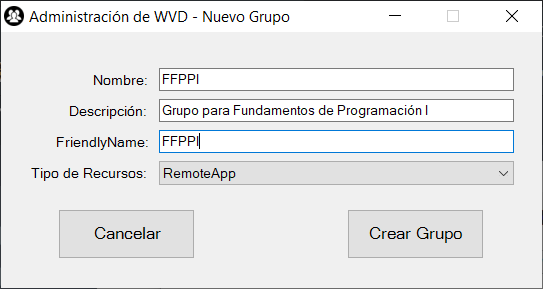
\includegraphics[width=0.6\linewidth]{figures/images/casos_uso/creacion_grupo_ffppi.PNG}
  \caption{Creación del grupo para FFPPI}
  \label{fig:cg_ffppi}
\end{figure}

Posteriormente, se seleccionan las aplicaciones que serán necesarias para impartir la asignatura y se proporciona acceso a los usuarios que lo requieran (Figura \ref{fig:params_ffppi}).

\begin{figure}[h]
  \centering
  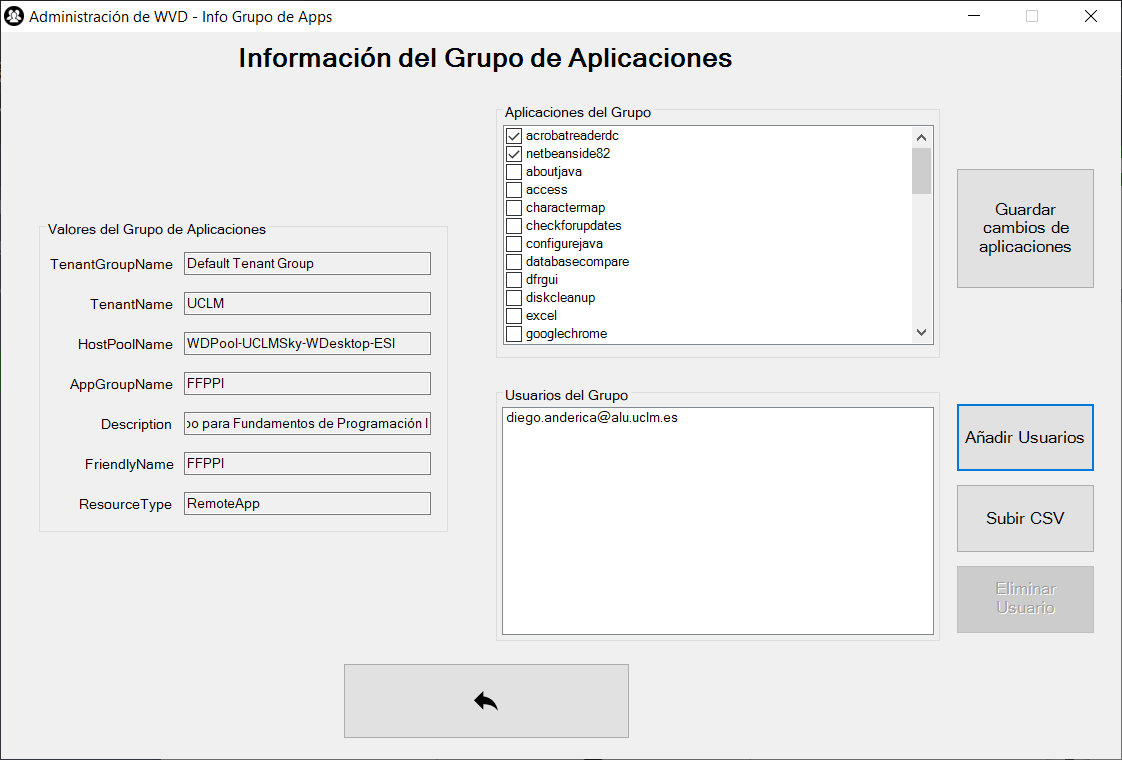
\includegraphics[width=0.8\linewidth]{figures/images/casos_uso/params_ffppi.PNG}
  \caption{Parámetros para FFPPI}
  \label{fig:params_ffppi}
\end{figure}

\clearpage

\subsubsection{Resultados y métodos de acceso}
Por último, se mostrarán los resultados finales tras realizar todos los pasos descritos anteriormente. Los usuarios podrán acceder a este servicio a través de la página web proporcionada por Microsoft a tal efecto (\url{https://rdweb.wvd.microsoft.com/webclient}) o utilizando el cliente de escritorio, disponible para Windows (\url{https://go.microsoft.com/fwlink/?linkid=2068602}). Por tanto, lo que el usuario visualizaría sería lo que se muestra en la Figura \ref{fig:web_alu}, en el caso de entrar a través de un navegador y como en la Figura \ref{fig:rd_alu}, en el caso de utilizar la aplicación de escritorio. Esta última, además, ofrece ciertas ventajas, como una menor latencia, la posibilidad de <<mapear>> el disco duro local para acceder a los archivos que se tengan guardados en el ordenador personal de una manera más sencilla y el hecho de mover las ventanas de los programas como si estos estuvieran instalados de manera nativa.

\begin{figure}[h]
  \centering
  
\includegraphics[width=0.8\linewidth]{figures/images/casos_uso/web_alu.PNG}
  \caption{Vista web de \acs{WVD}}
  \label{fig:web_alu}
\end{figure}

\begin{figure}[h]
  \centering
  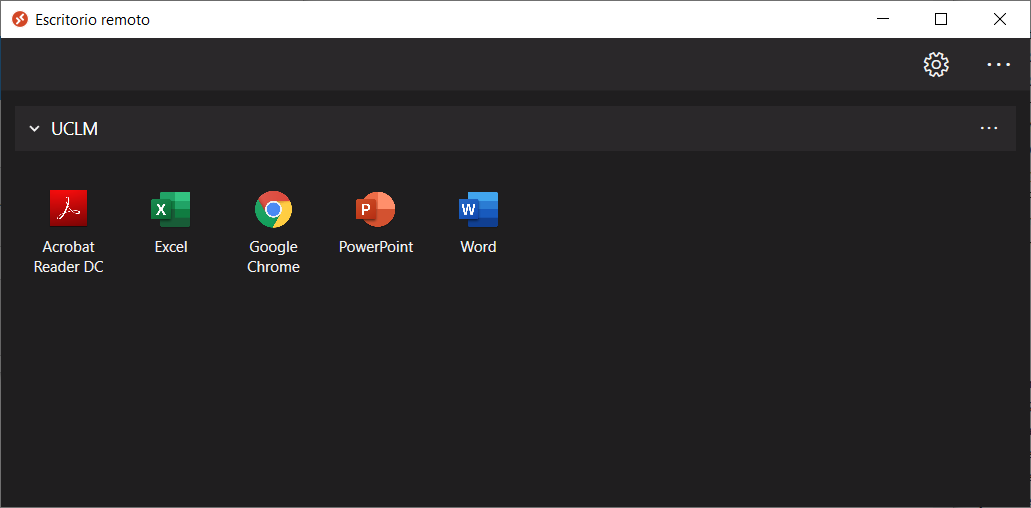
\includegraphics[width=0.8\linewidth]{figures/images/casos_uso/rd_alu.PNG}
  \caption{Vista de app nativa}
  \label{fig:rd_alu}
\end{figure}

\clearpage

\subsection{Costes del servicio y estudio comparativo}
Por último, una vez que se ha comprobado la viabilidad de la implementación y entrega del servicio, se realizará un pequeño análisis y estudio comparativo donde se enfrente el coste aproximado de los recursos y el coste de adquisición de equipos teniendo en cuenta los casos de uso desarrollados.

\subsubsection{Coste de los recursos \textit{cloud} (caso 1)}

Para realizar los cálculos del coste del caso 1 se han tomado los datos que la \acs{UCLM} proporciona a través de la página web. Según su portal de transparencia \cite{uclmstats}, durante el curso 2018-2019 hubo un total de 2.659 alumnos matriculados en títulos propios. Por tanto, realizando una estimación de equipos denominados como de <<libre uso>> de un 10\% en relación al total de alumnos, habría alrededor de unos \textbf{266 puestos de trabajo} (se utilizarán 300 para los cálculos) a disposición de los estudiantes durante las horas laborables. Para obtener el total aproximado de horas, se ha tomando el horario de apertura de la biblioteca general de la \acs{UCLM} del campus de Ciudad Real para este año 2019 \cite{horariobib} y se ha extraído una relación con las horas de apertura aproximadas en un año (Tabla \ref{tab:relhorasbib}).

\begin{table}[!htbp]
	\centering
	{\small
		\begin{tabular}{|c|c|c|c|}
\hline
\rowcolor[HTML]{343434} 
{\color[HTML]{FFFFFF} \textbf{Horario de apertura}} & {\color[HTML]{FFFFFF} \textbf{Horas diarias}} & {\color[HTML]{FFFFFF} \textbf{Días}} & {\color[HTML]{FFFFFF} \textbf{Horas}} \\ \hline
08:30 - 04:00 & 19,5 & 58  & 1.131 \\ \hline
08:30 - 21:00 & 12,5 & 129 & 1.613 \\ \hline
09:00 - 21:00 & 12   & 6   & 72    \\ \hline
09:00 - 20:00 & 11   & 10  & 110   \\ \hline
09:00 - 04:00 & 19   & 26  & 494   \\ \hline
09:00 - 14:00 & 5    & 27  & 135   \\ \hline
Cerrada       & -    & 109 & 0     \\ \hline
\multicolumn{3}{|r|}{\cellcolor[HTML]{343434}{\color[HTML]{FFFFFF} \textbf{TOTAL HORAS}}}                                                  & \textbf{3.555 \textasciitilde{} 4.000}                        \\ \hline
\end{tabular}
	}
	\caption[Relación horas apertura biblioteca]
	{Relación horas apertura biblioteca}
	\label{tab:relhorasbib}
\end{table}

\clearpage

A continuación, se ha recurrido a la calculadora de precios que ofrece Microsoft en la web de Azure \cite{calculadoraAzure} para realizar un presupuesto aproximado. Para ello, se han añadido los elementos que han sido necesarios para construir los casos de uso: una máquina virtual para realizar la plantilla y el propio servicio de \acs{WVD}.

Para la máquina virtual, se ha elegido la región de Europa Occidental, con sistema operativo Windows y una instancia B2MS, que tendrá la capacidad suficiente para realizar las tareas de instalación de las herramientas necesarias. Como opción de facturación se ha elegido pago por uso con una máquina virtual durante un día al mes, tiempo que se estima suficiente para poder instalar dichas herramientas holgadamente, así como para realizar modificaciones cuando se requiera. En cuanto al almacenamiento, se ha seleccionado un disco duro estándar con un tamaño de 128 \acs{GB} y las unidades de transacción por defecto (100). El precio resultante de esta parte de la configuración es el que se muestra en la Figura \ref{fig:presu_mv}: unos 7,11\euro{}.

Por otra parte, en el caso del servicio de \acs{WVD}, se ha seleccionado de nuevo Europa Occidental como región con el servicio del tipo \textit{pooled}. Esto significa que, dependiendo de las circunstancias, un usuario podría acceder aleatoriamente a cualquiera de las máquinas disponibles, sin ocupar una entera. En cuanto al número de usuarios, como se ha comentado anteriormente, se ha fijado a 300 con un pico máximo del 90\%, un mínimo del 5\% y unas 350 horas de uso al mes (4.000/12 = 333,34 \textasciitilde{} 350). Este servicio representaría un escenario multisesión para un mejor aprovechamiento de los recursos y una carga de trabajo ligera. Con esta configuración, el tipo de máquina virtual recomendado es D8S v3. Para una primera prueba, la opción de facturación será de pago por uso aunque, de continuar con el servicio, sería más económico reservar las máquinas virtuales por uno o tres años. Por último, el almacenamiento será de discos duros estándar de 128 \acs{GB}, resultando en un presupuesto mensual aproximado de 1.033,66\euro{} (Figura \ref{fig:presu_WVD}).

Por tanto, el coste aproximado de los recursos y el servicio de \acs{WVD} en Azure para prestar un servicio ligero como es el de las aulas de libre uso sería de unos 1.040,77\euro{} \textasciitilde{} 1.050\euro{} mensuales.

\begin{figure}[h]
  \centering
  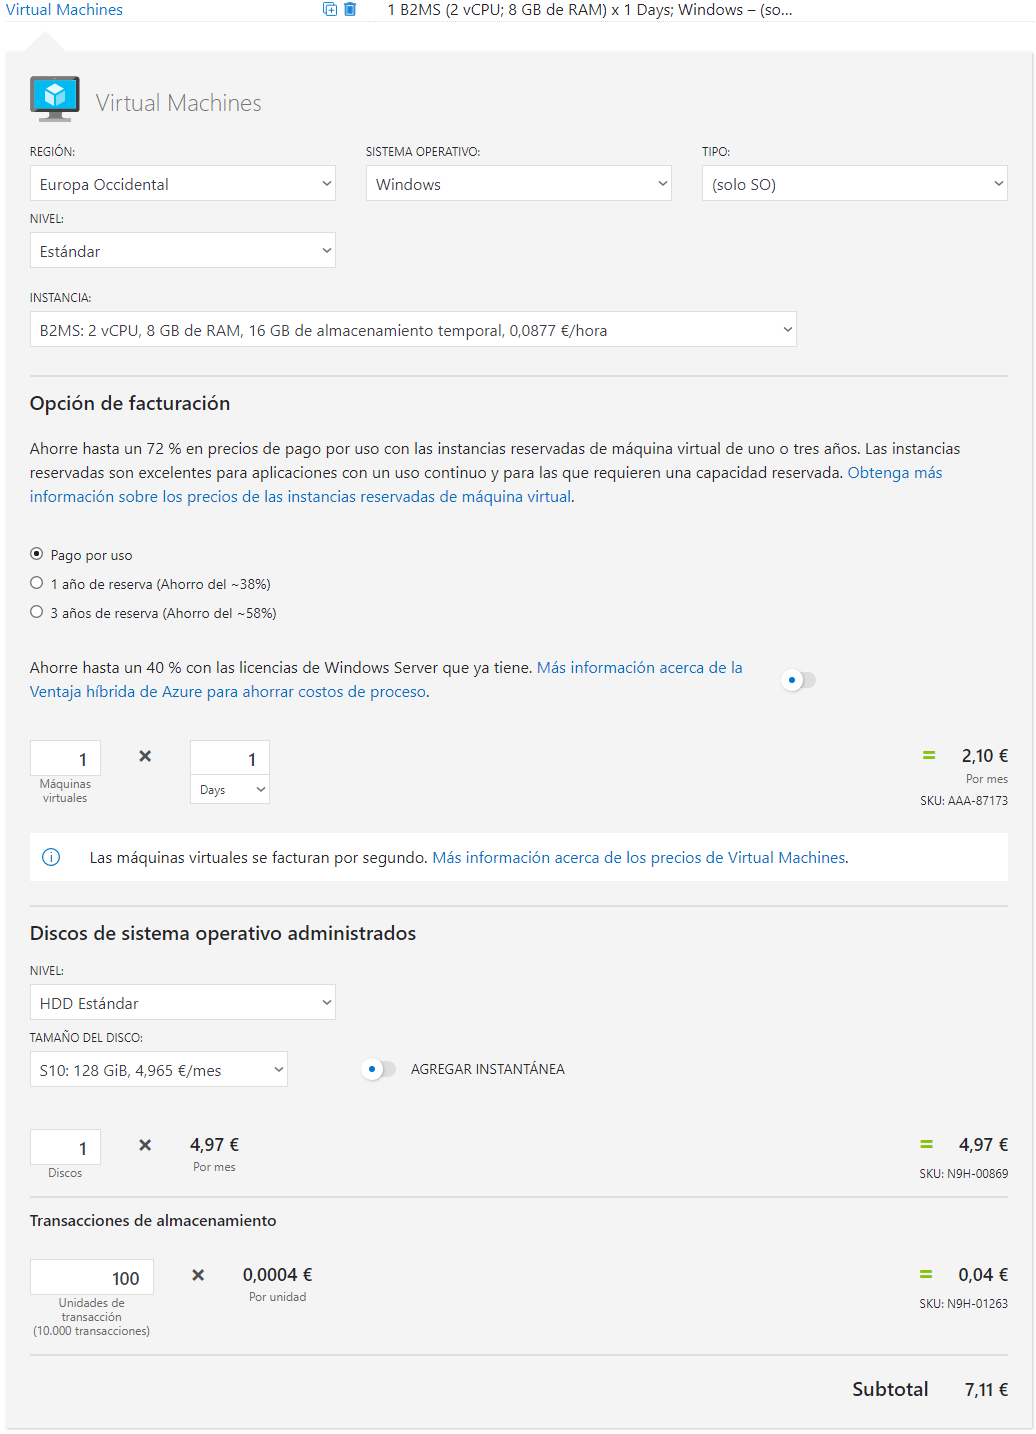
\includegraphics[width=0.9\linewidth]{figures/images/presupuesto/presu_mv.png}
  \caption{Presupuesto de máquina virtual}
  \label{fig:presu_mv}
\end{figure}

\begin{figure}[h]
  \centering
  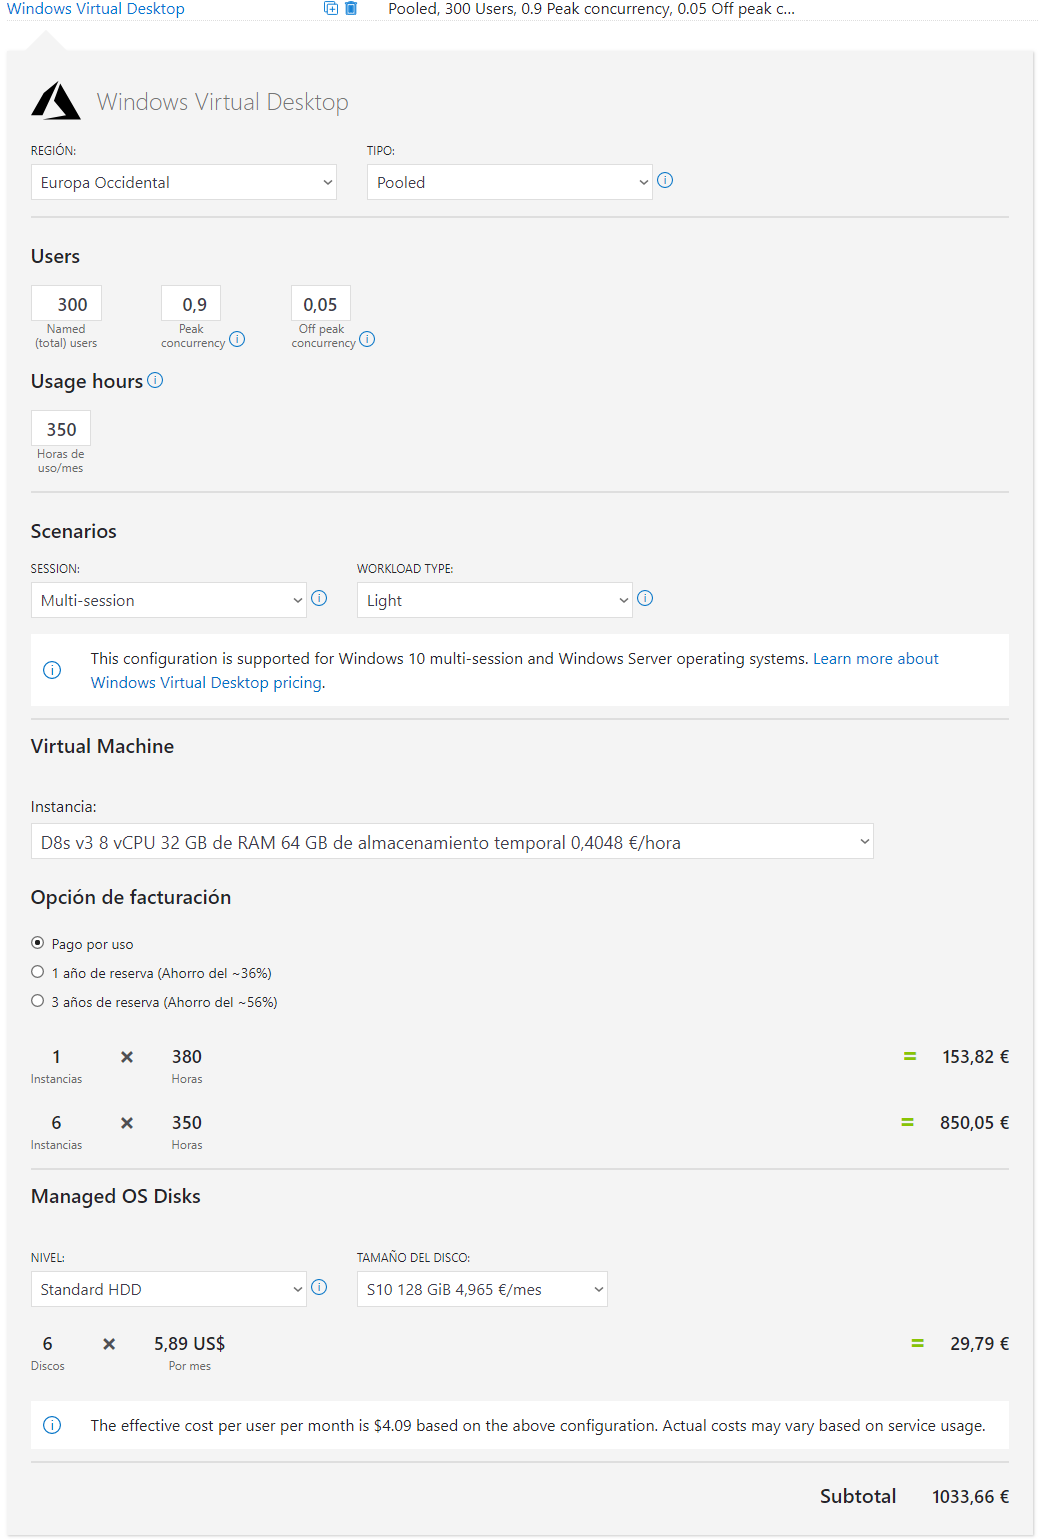
\includegraphics[width=0.9\linewidth]{figures/images/presupuesto/presu_wvd.png}
  \caption{Presupuesto de \acs{WVD} (caso 1)}
  \label{fig:presu_WVD}
\end{figure}

\clearpage

\subsubsection{Coste de los recursos \textit{cloud} (caso 2)}
En cuanto al segundo caso realizado para la asignatura de Fundamentos de Programación I, se han estimado de igual manera los costes aproximados de los recursos \textit{cloud}. Al ser una asignatura cuatrimestral con un peso de seis créditos \acs{ECTS} (150 horas), se realizarán los cálculos para cuatro meses. Por tanto, el servicio se utilizaría unas 37,5 horas \textasciitilde{} 50 horas al mes.

En todos los casos deberá haber una máquina virtual en la que se instalen las herramientas por lo que, en esta ocasión, se dispondría de una máquina con las mismas características que la mostrada en la Figura \ref{fig:presu_mv}. No obstante, en el caso del servicio de \acs{WVD}, algunos de los parámetros como el de número de usuarios y las horas de uso al mes varían, fijándose en 150 y 50, respectivamente. Esto arroja un coste total de 350,87\euro{} (Figura \ref{fig:presu_WVD2}).

Por tanto, atendiendo al coste de la máquina para realizar la plantilla (7,11\euro{}) y al coste del servicio de \acs{WVD} para 150 estudiantes durante 50 horas al mes con una carga de trabajo ligera (350,87\euro{}), el precio total de los recursos \textit{cloud} ascendería a unos 360\euro{} al mes, aproximadamente (1440\euro{} por cuatrimestre).

\begin{figure}[h]
  \centering
  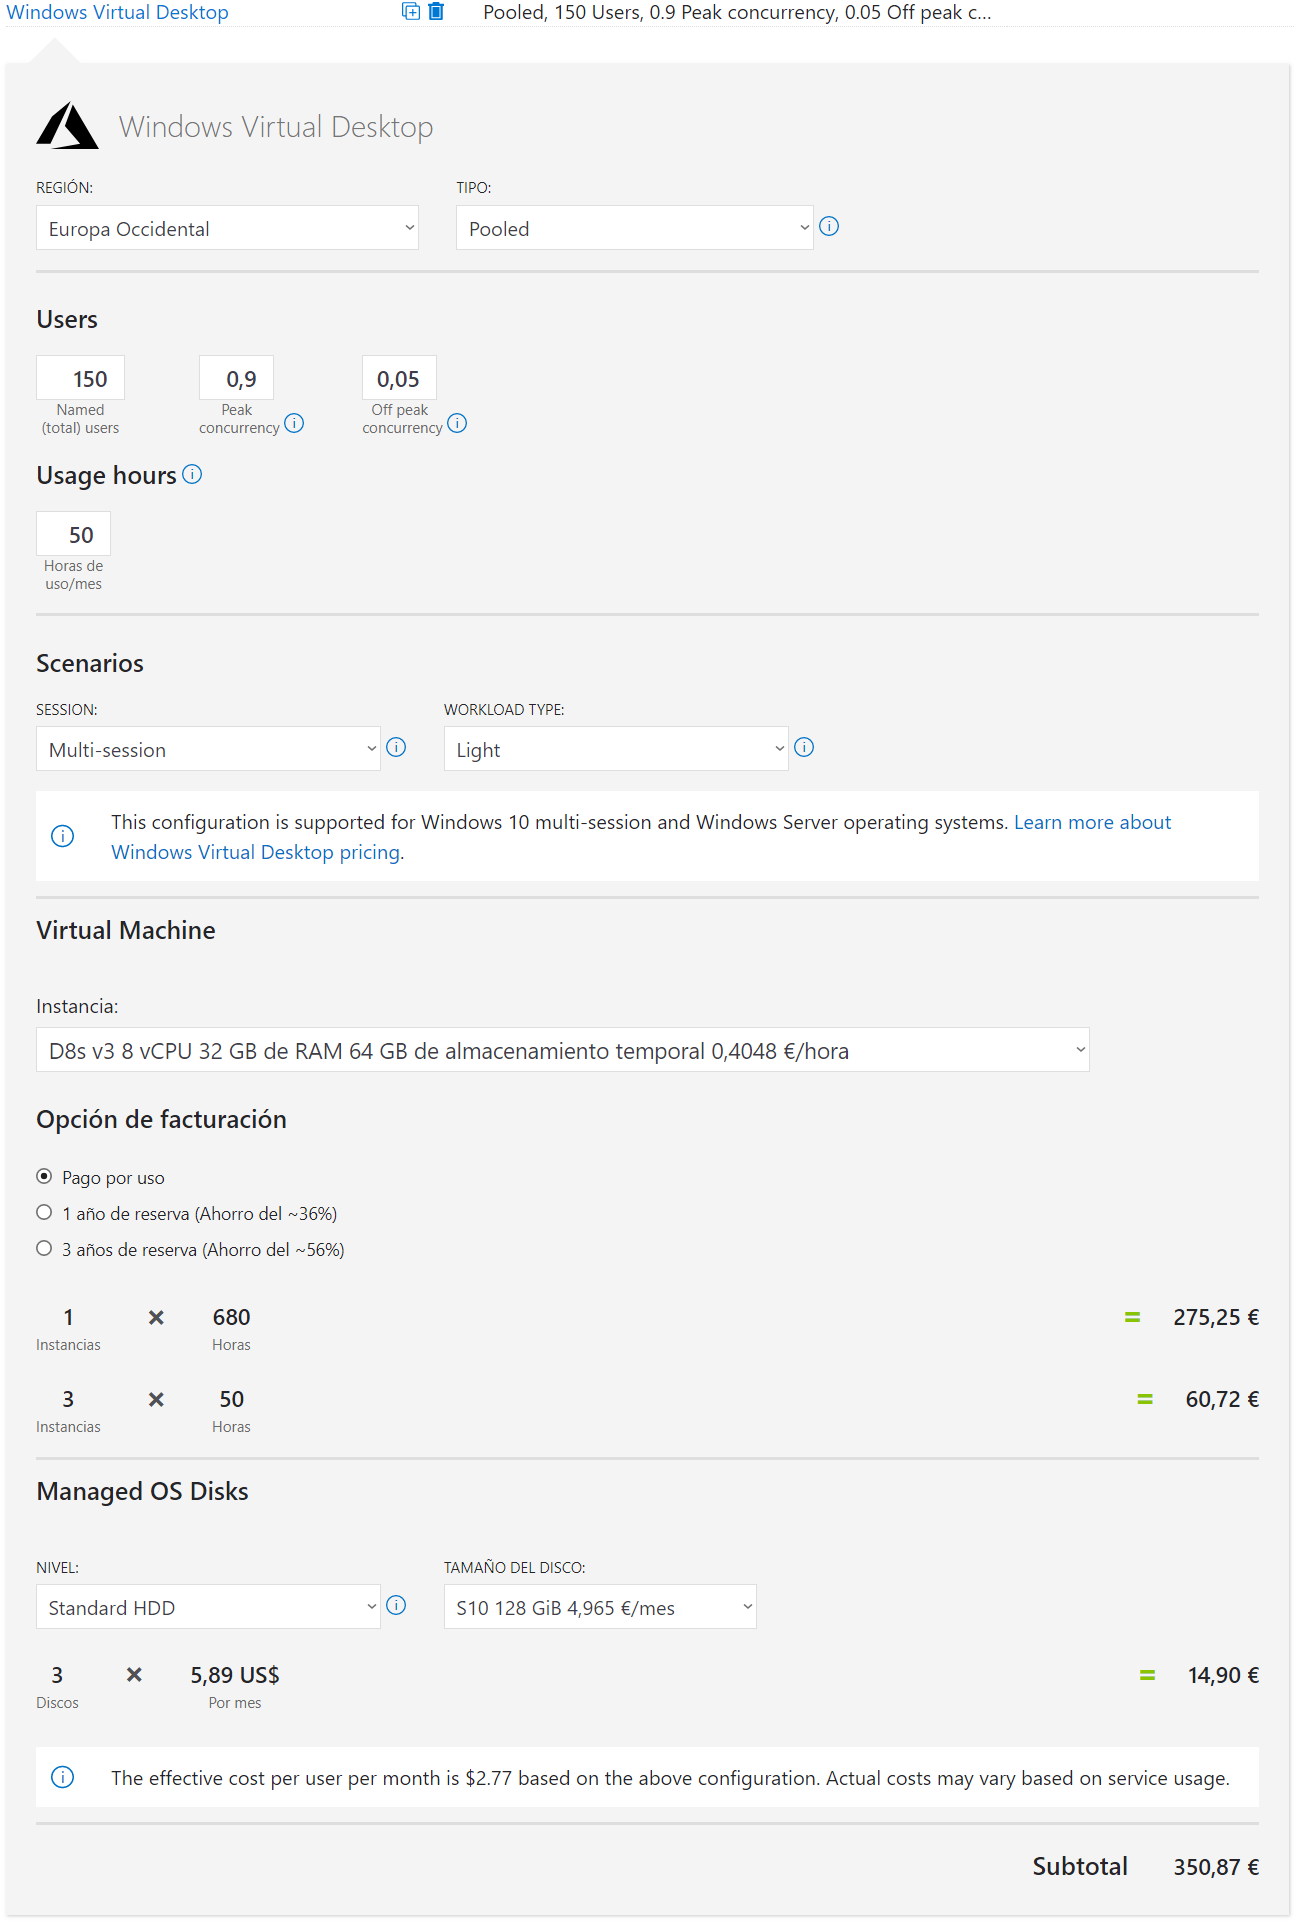
\includegraphics[width=0.9\linewidth]{figures/images/presupuesto/presu_wvd2.png}
  \caption{Presupuesto de \acs{WVD} (caso 2)}
  \label{fig:presu_WVD2}
\end{figure}

\clearpage

\subsubsection{Coste de adquisición de equipos}
Poniendo el foco en el coste de adquisición de los equipos, se ha tomado como ejemplo el modelo 600 G3 \acf{AIO} de HP, homologado en la universidad e ideado para equipamiento de aulas (Figura \ref{fig:hp_aio}). Su coste es de 669\euro{} + \acs{IVA}, lo que lo situaría en alrededor de 800\euro{}. En el caso de que hubiera que realizar una compra para 150 puestos tendría un coste de 120.000\euro{}, cantidad suficiente para disponer del servicio del caso 2 durante unos 83 cuatrimestres. En el caso de que se adquiriera uno para cada dos estudiantes, tendría un coste de alrededor de 60.000\euro{}, equivalente al coste del servicio durante unos 41 cuatrimestres.

\begin{figure}[h]
  \centering
  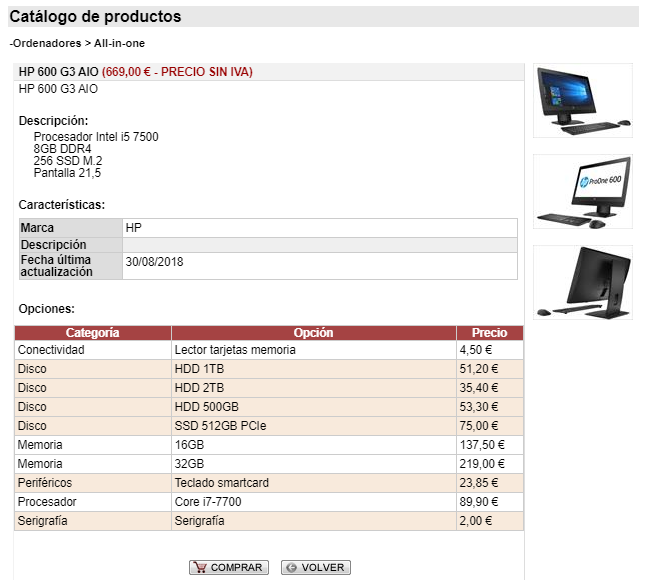
\includegraphics[width=0.8\linewidth]{figures/images/presupuesto/aio_hp.png}
  \caption{HP 600 G3 \acs{AIO}}
  \label{fig:hp_aio}
\end{figure}

Por tanto, cuando se toman valores realistas del servicio y se enfrentan a los costes de adquisición de hardware, es posible contrastar ambos para tomar una mejor decisión. Además, el uso del servicio de \acs{WVD} asegura que no se desaprovechan recursos, sino que la capacidad de cómputo se ajusta a las necesidades en cualquier escenario concreto con la ventaja de que, con una periodicidad establecida, los componentes \textit{cloud} son renovados, evitando así la obsolescencia.